\section[Online/Real-time Analysis]{Online Analysis}
\label{sec:online}

On similar lines as \cite{ghanvati01, sanchez01}, test were conducted for checking if the symptoms of Critical Slowing Down could  be detected by a real-time/online analysis of the state variables of a power grid. In other words, can computing the autocorrelation and variance of real-time PMU data processed over a running window function appropriately as Early Warning Signs of an impending approach instability.

Bifurcation Theory states that a small change in system parameters, such the governor reference power for a generator ($P_{Gen}$) at certain points, can lead to major upsets in the stability of the power grid. We ran a simulation in which a system was purposefully stressed (via a near constant linear load increment) as time progressed but many restrictions/safety mechanisms were lifted with the aim of singling-out the cause of bifurcation to a change in $P_{Gen}$(s), in order to best demonstrate that the proposed statistical mechanisms (computing autocorrelations and variances) function well as Early Warning Signs even for slow and steady variations of loads, and not just for sudden changes in state variables caused due to reactionary corrective protection mechanisms or the machines not being given `free-range' for chasing load increments due to specified safety limits on maximum allowed generated powers. Below is the set of special conditions used for the simulation of the IEEE 9 Bus system:

\begin{enumerate}
	\item The three load points of the system (Buses 5, 6 and 8) were linearly increased in time, at a rate of $\Delta P \%$ per minute plus a small white noise component $\mathcal{N}(0, \sigma_v)$, with every increment happening at $\Delta t$ time intervals. 
	\begin{equation}
		P_{L_i}(t+\Delta t) = P_{L_i}(t)*\left(1+ \frac{\Delta P_{L_i}}{100}\right) + \mathcal{N}(0, \sigma_v)
	\end{equation} 
	Here, $\Delta P_{L}$ values were assigned randomly between $8-12\%$ for every load bus, $\sigma_v = 0.01$ and $\Delta t = 0.1$ seconds.
	\item Simulation ODE solver solves for the new state variables for the system every $0.01$ seconds. This means that the simulation output can be likened to a stream of PMU data whose sampling rate is $100$ Hz.
	\item Protection mechanisms were disabled. No remedial/corrective action was taken for any drop in bus voltages/grid frequency or any increase in line currents/MVAs.
	\item `Dummy' governors were placed on the three generators (at buses 1, 2 and 3) which could respond instantly to load changes by changing the set reference generation powers $P_{Gen}$(s) with zero time lag.
	\item The generator limits for $P_{Gen_{MAX}}$, $Q_{Gen_{MAX}}$, etc. were removed. Thus the generators had complete freedom to `chase' the load increments at the load buses, including factoring in the extra line-losses.
\end{enumerate} 

Based on the above conditions, simulations were run in PSSE. The simulations ran for about two minutes before the grid `blacked out' i.e. PSSE solver returned the message `Network Not Converged' as the continuously increasing loads could not be handled by the generators while maintaining synchronism. The outputs of the state variables, including Demand/Load Powers, Generated Powers, Bus Frequencies, Bus Voltages, Line Currents and Line MVAs have been presented below in Figure \ref{fig:psse_run02}.

\begin{figure}[!ht]
	\centering
	\begin{subfigure}{\textwidth}
		\centering
		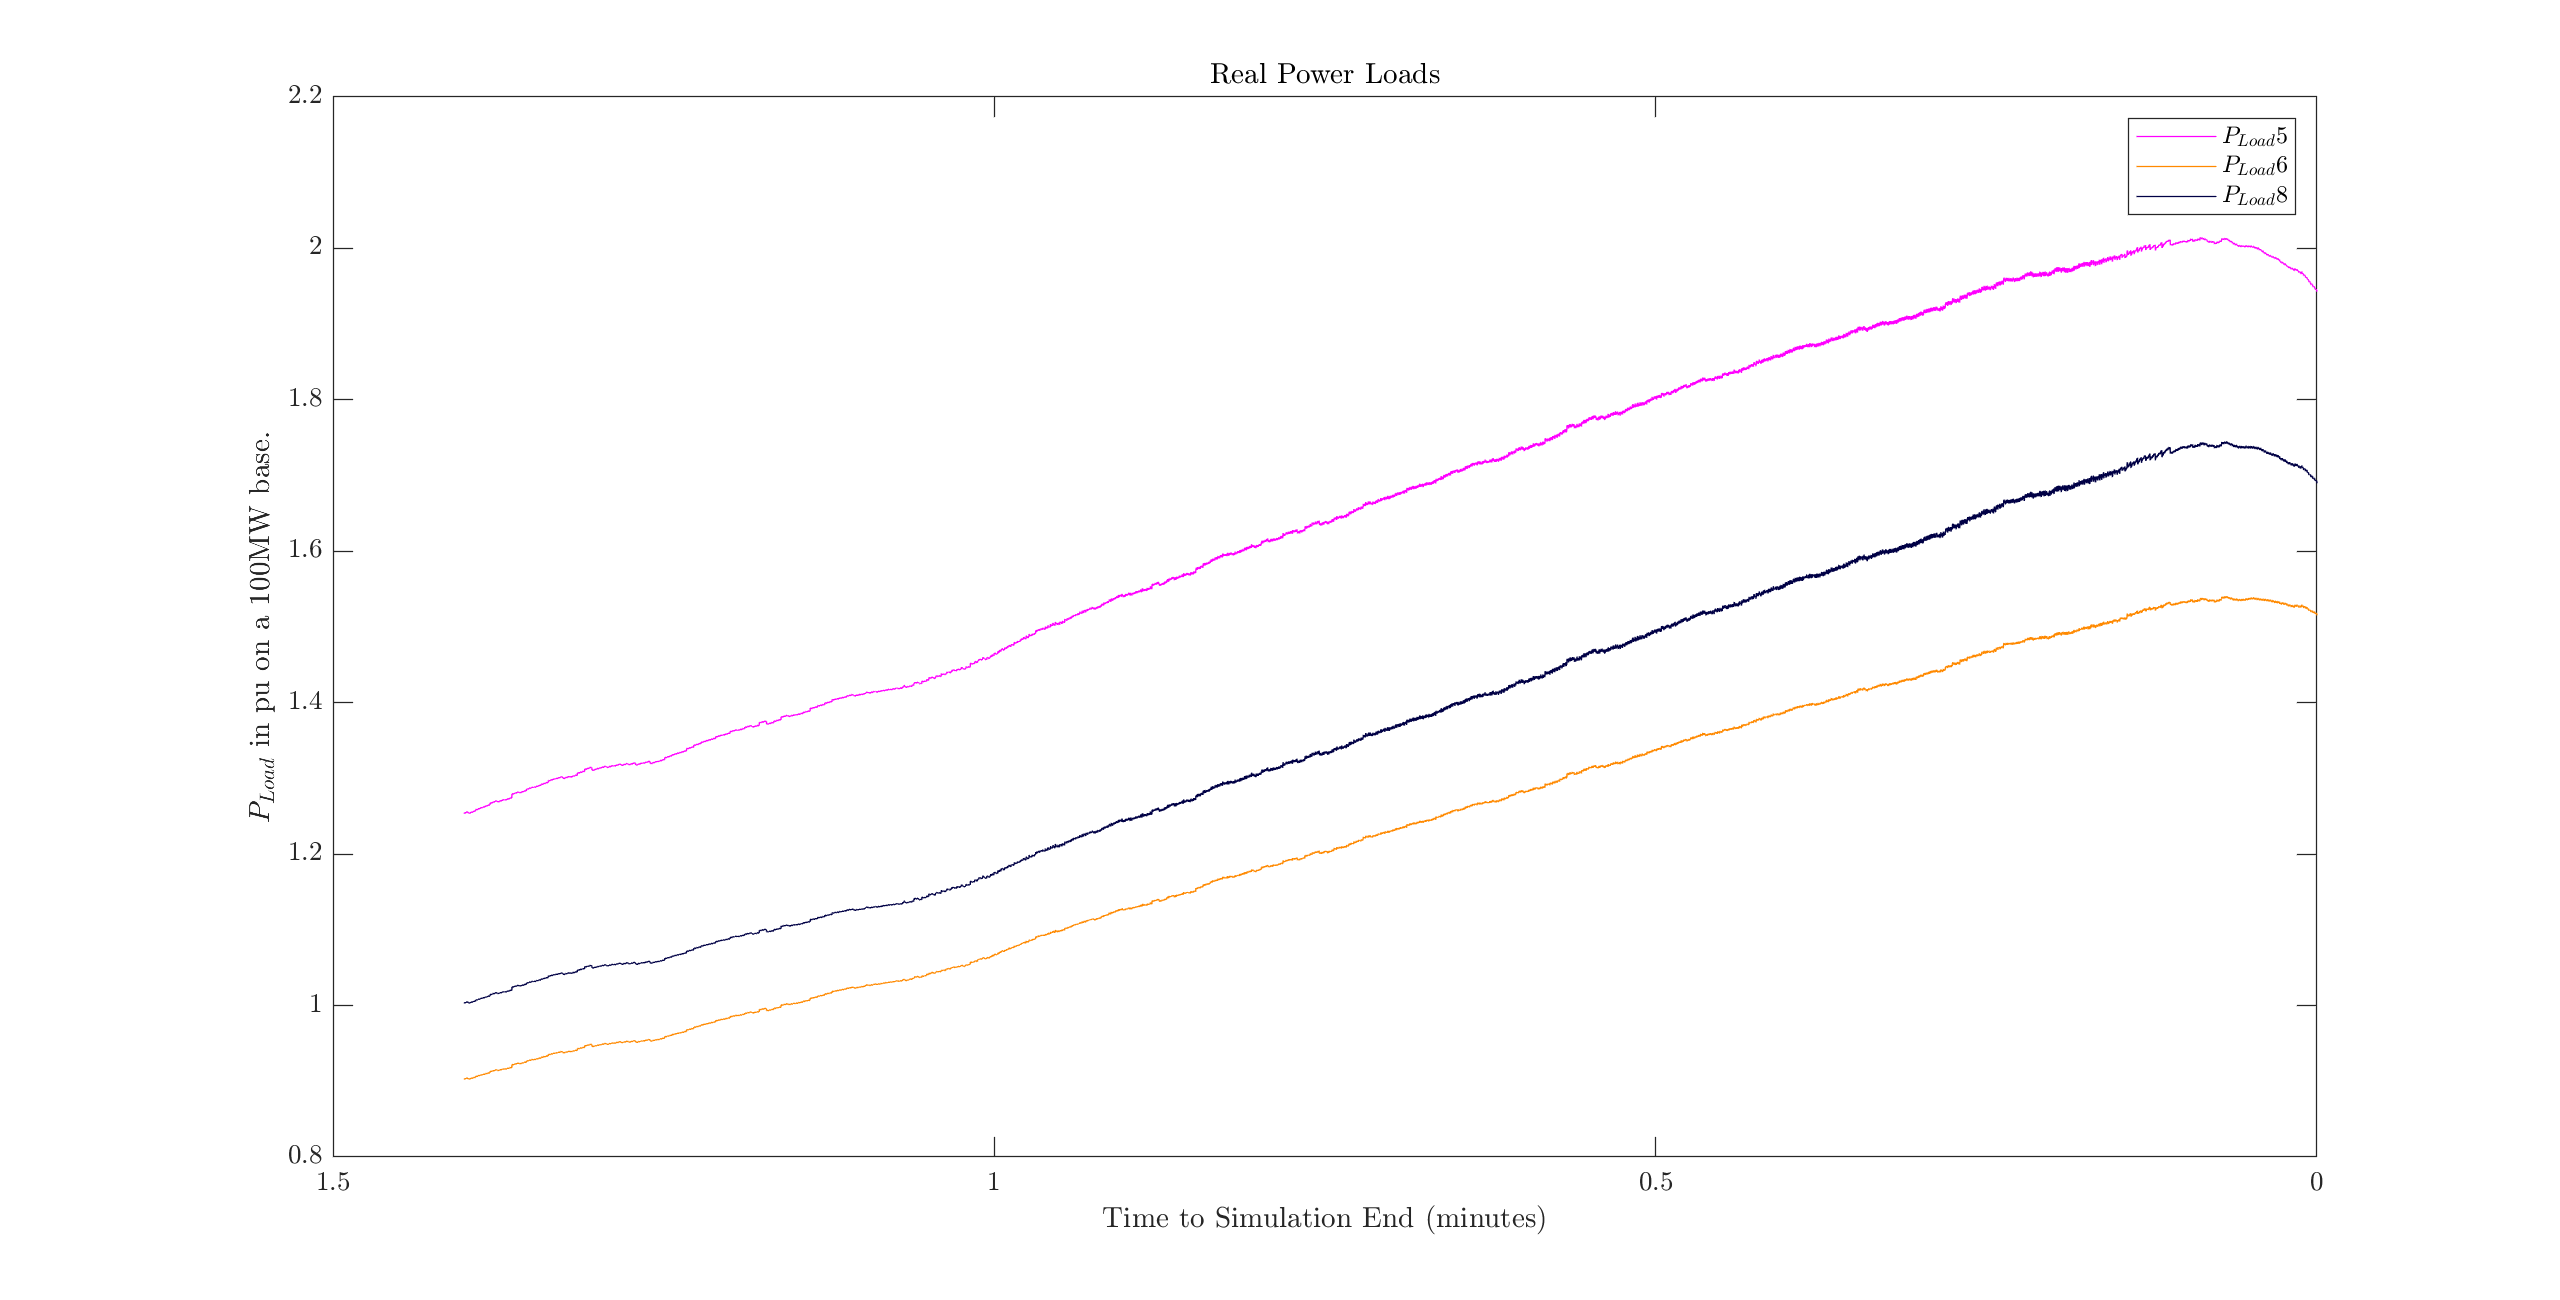
\includegraphics[scale=0.25]{../figures/analysis_matlab/ploads_run02}
		\caption{Real Power Loads for the simulated IEEE 9 Bus System vs simulation time.}
	\end{subfigure}
	
	\begin{subfigure}{\textwidth}
		\centering
		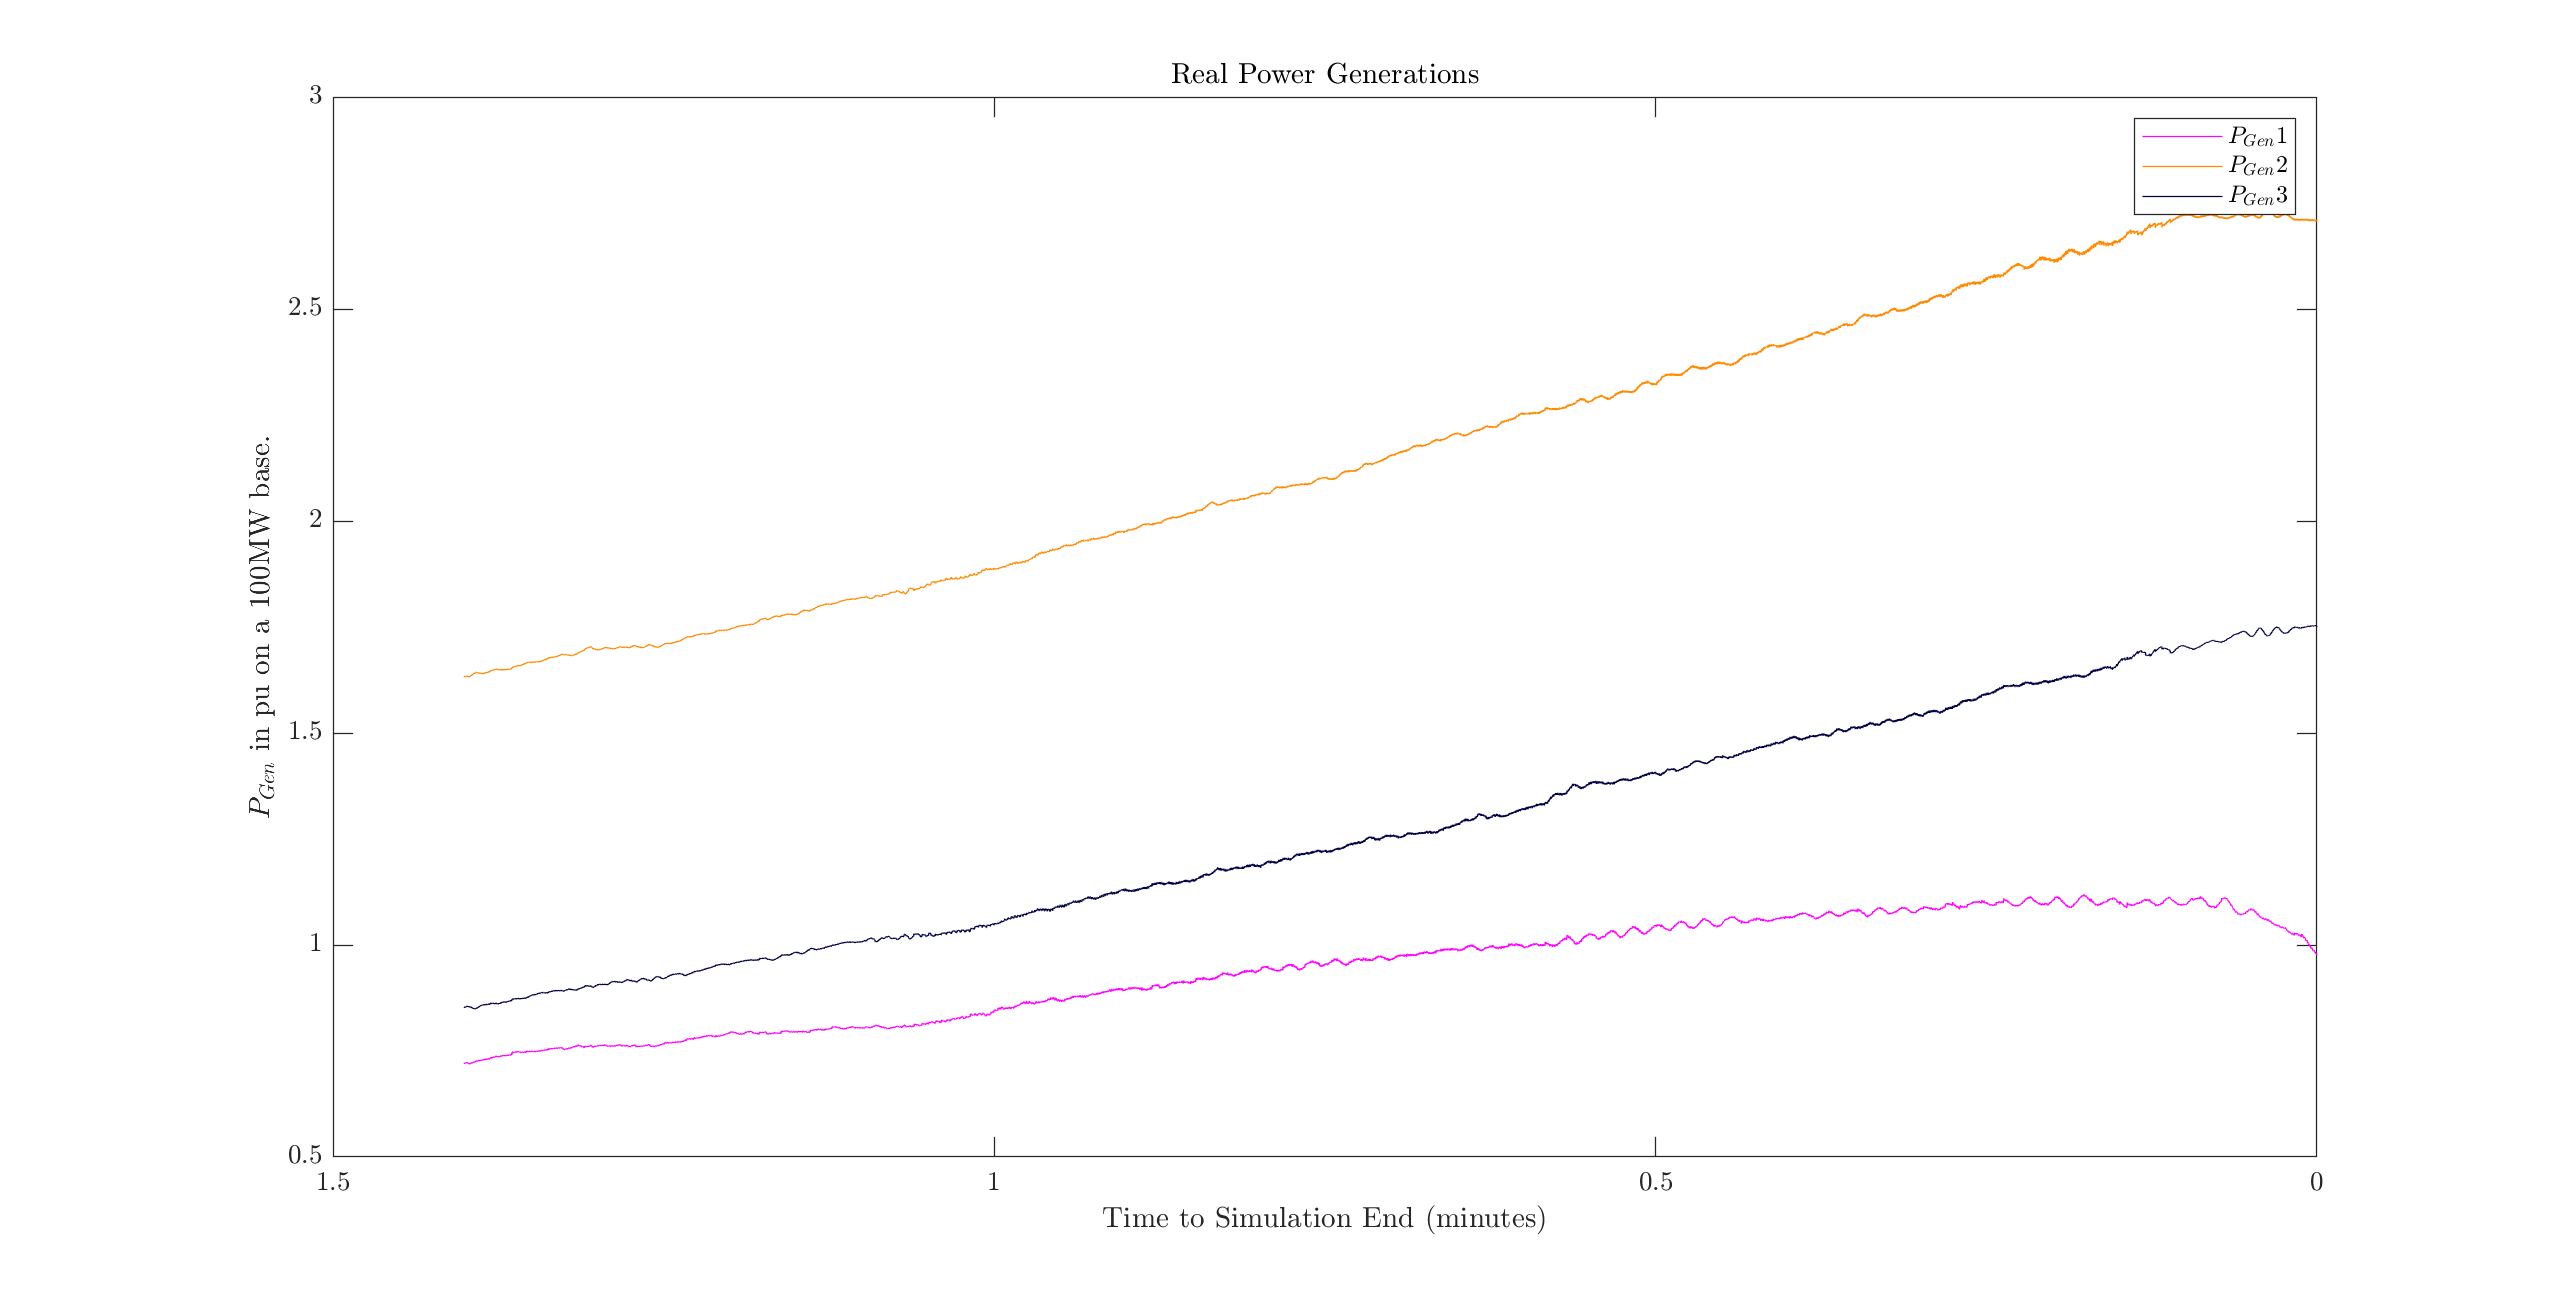
\includegraphics[scale=0.25]{../figures/analysis_matlab/pgens_run02}
		\caption{Generated Real Powers for the simulated IEEE 9 Bus System vs simulation time.}
	\end{subfigure}

	\caption{Simulation results of the IEEE 9 Bus System as per the prescribed conditions.}
	\label{fig:psse_run02}
\end{figure}

\begin{figure}[!htpb]
	\centering
	\begin{subfigure}{\textwidth}
		\centering
		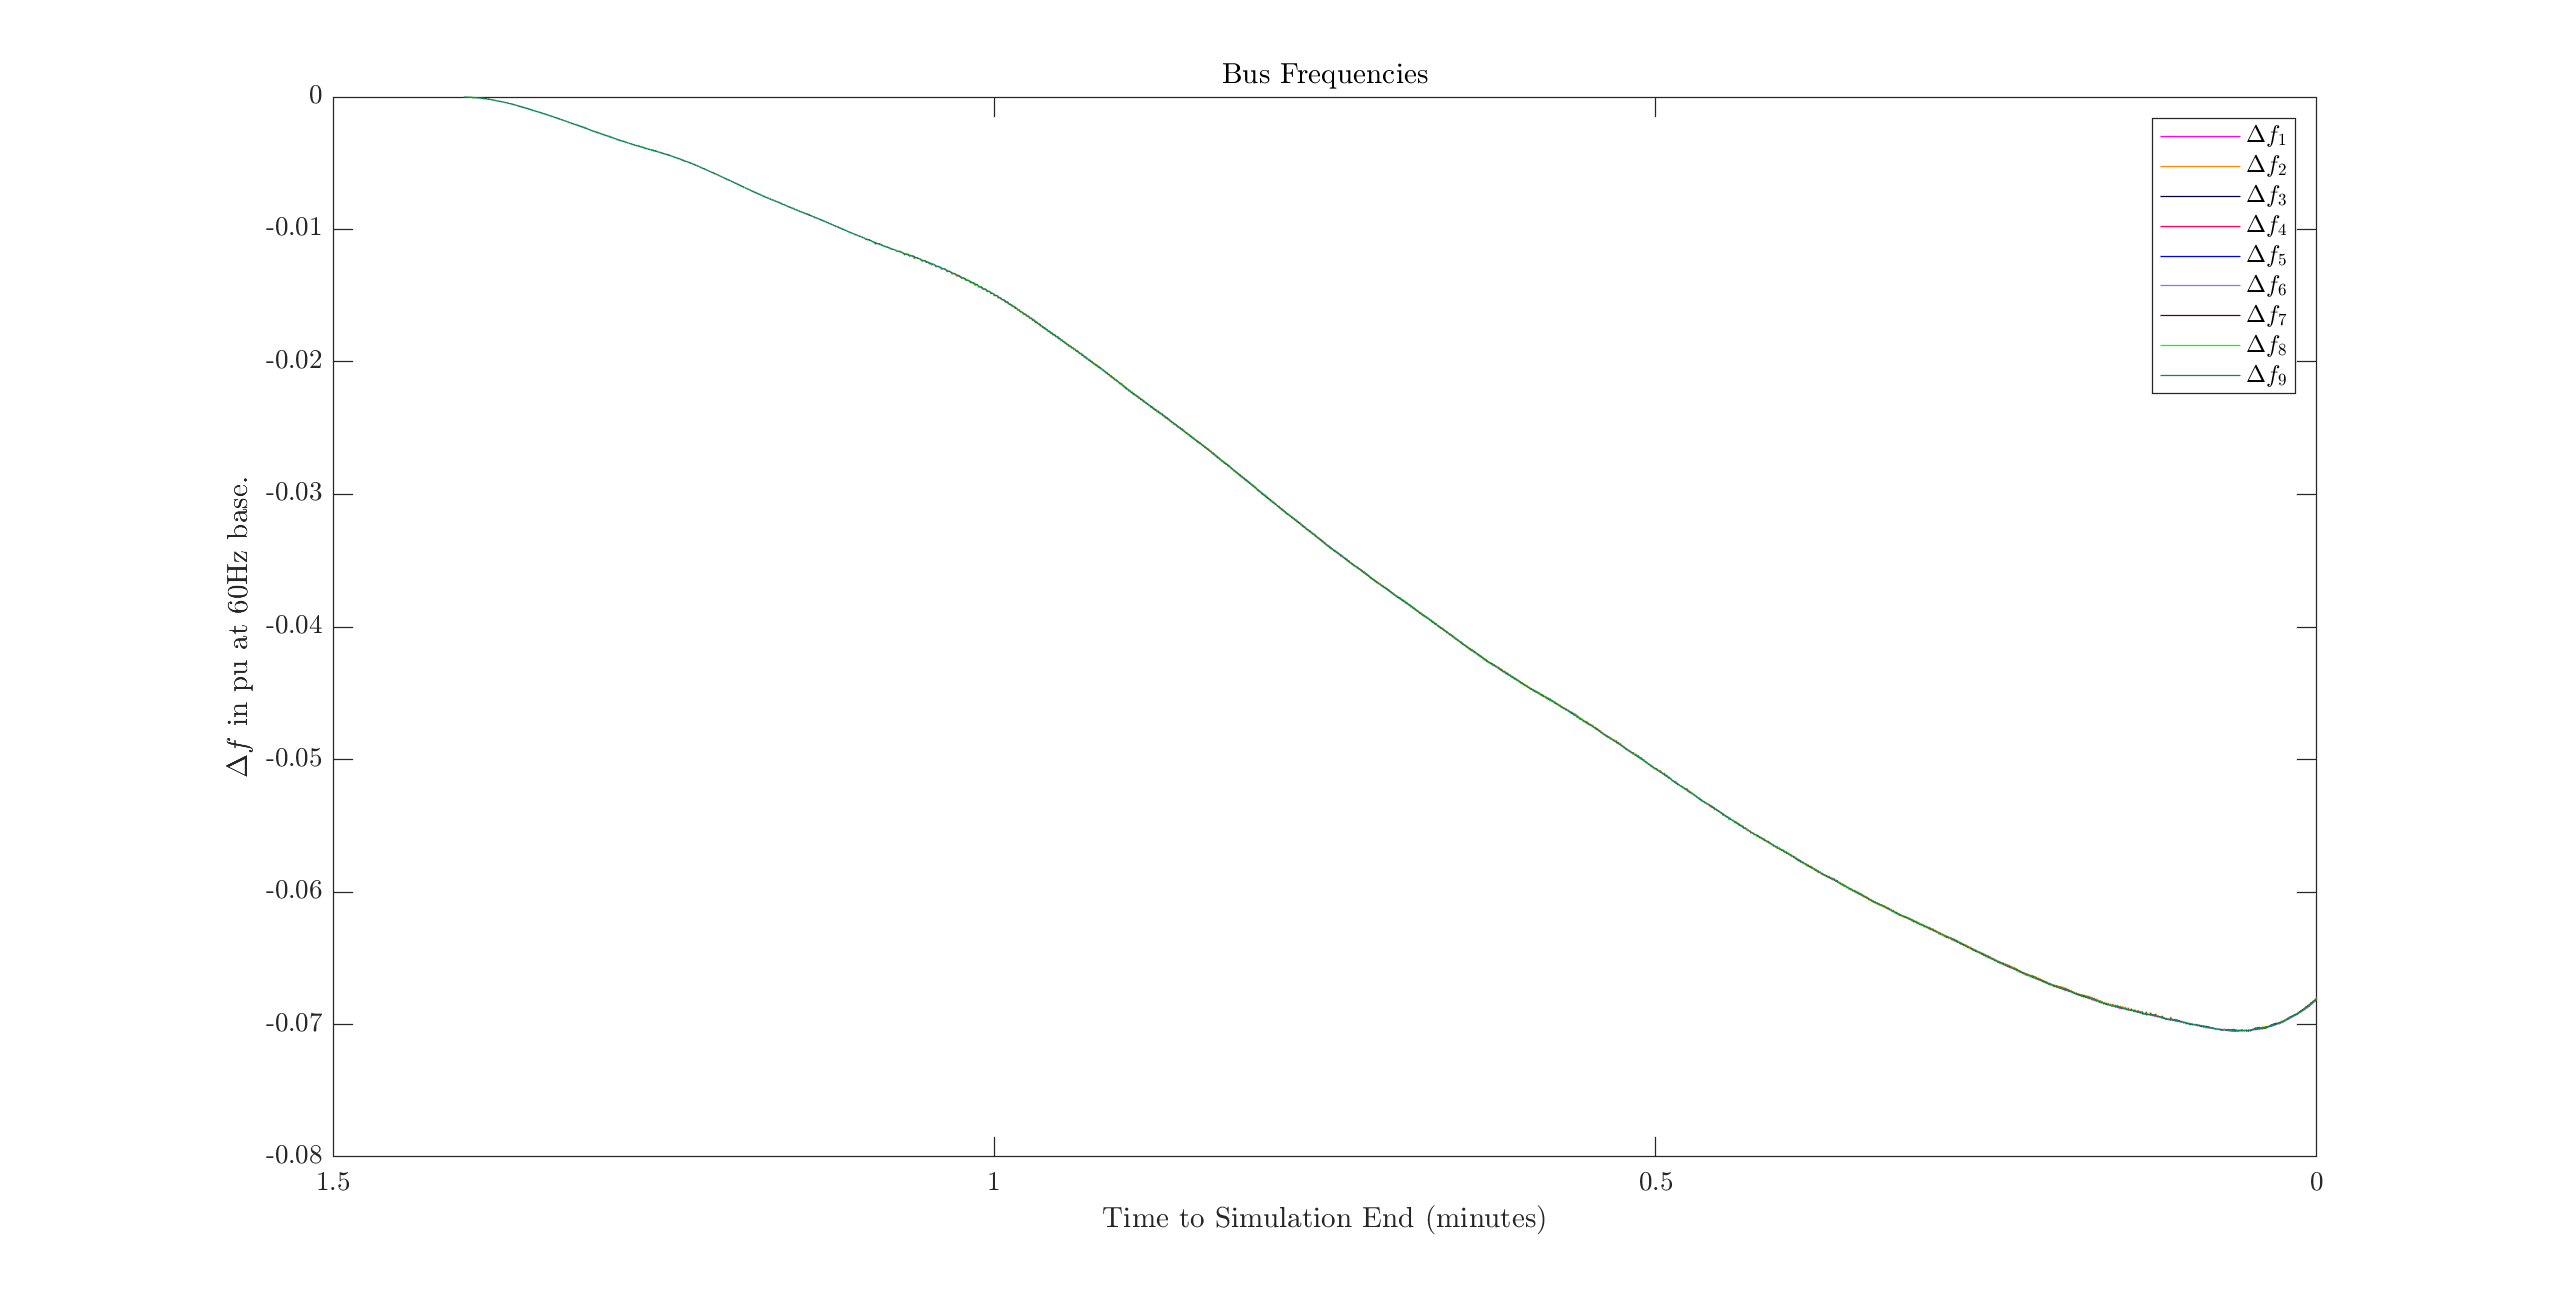
\includegraphics[scale=0.25]{../figures/analysis_matlab/frequencies_run02}
		\caption{Bus Frequencies for the simulated IEEE 9 Bus System vs simulation time.}
	\end{subfigure}
	
	\begin{subfigure}{\textwidth}
		\centering
		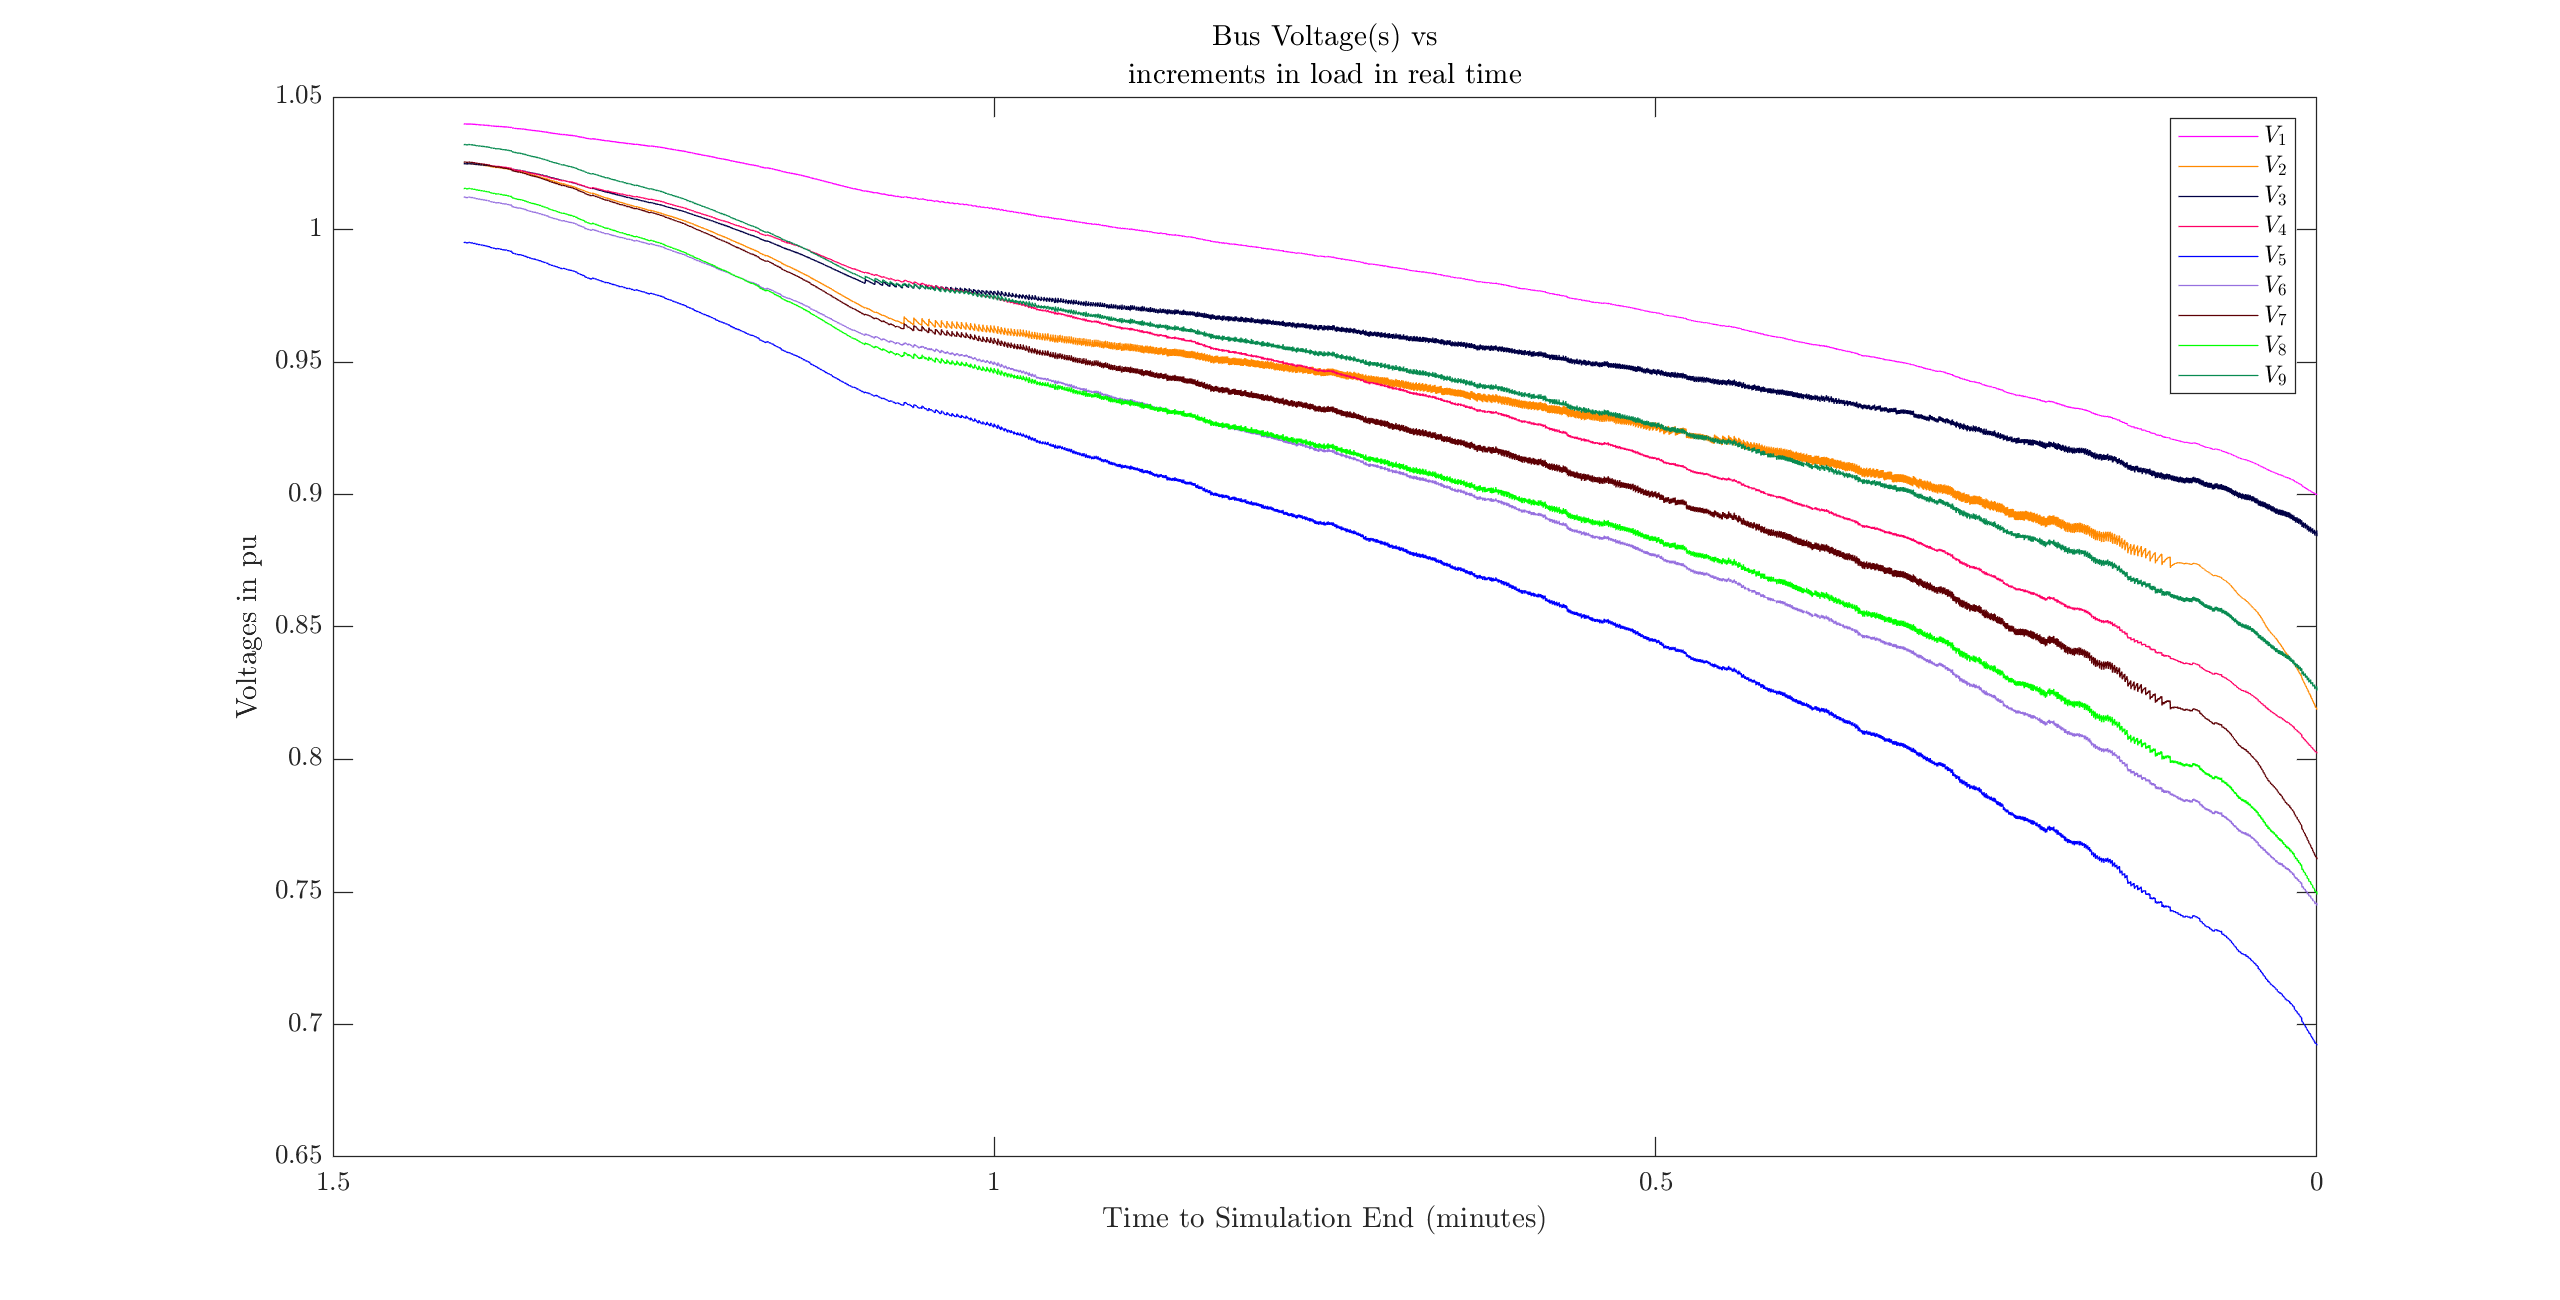
\includegraphics[scale=0.25]{../figures/analysis_matlab/voltages_run02}
		\caption{Bus Voltages for the simulated IEEE 9 Bus System vs simulation time.}
	\end{subfigure}

	\caption{Simulation results of the IEEE 9 Bus System as per the prescribed conditions.}
\end{figure}

\begin{figure}[!htpb]
	\begin{subfigure}{\textwidth}
		\centering
		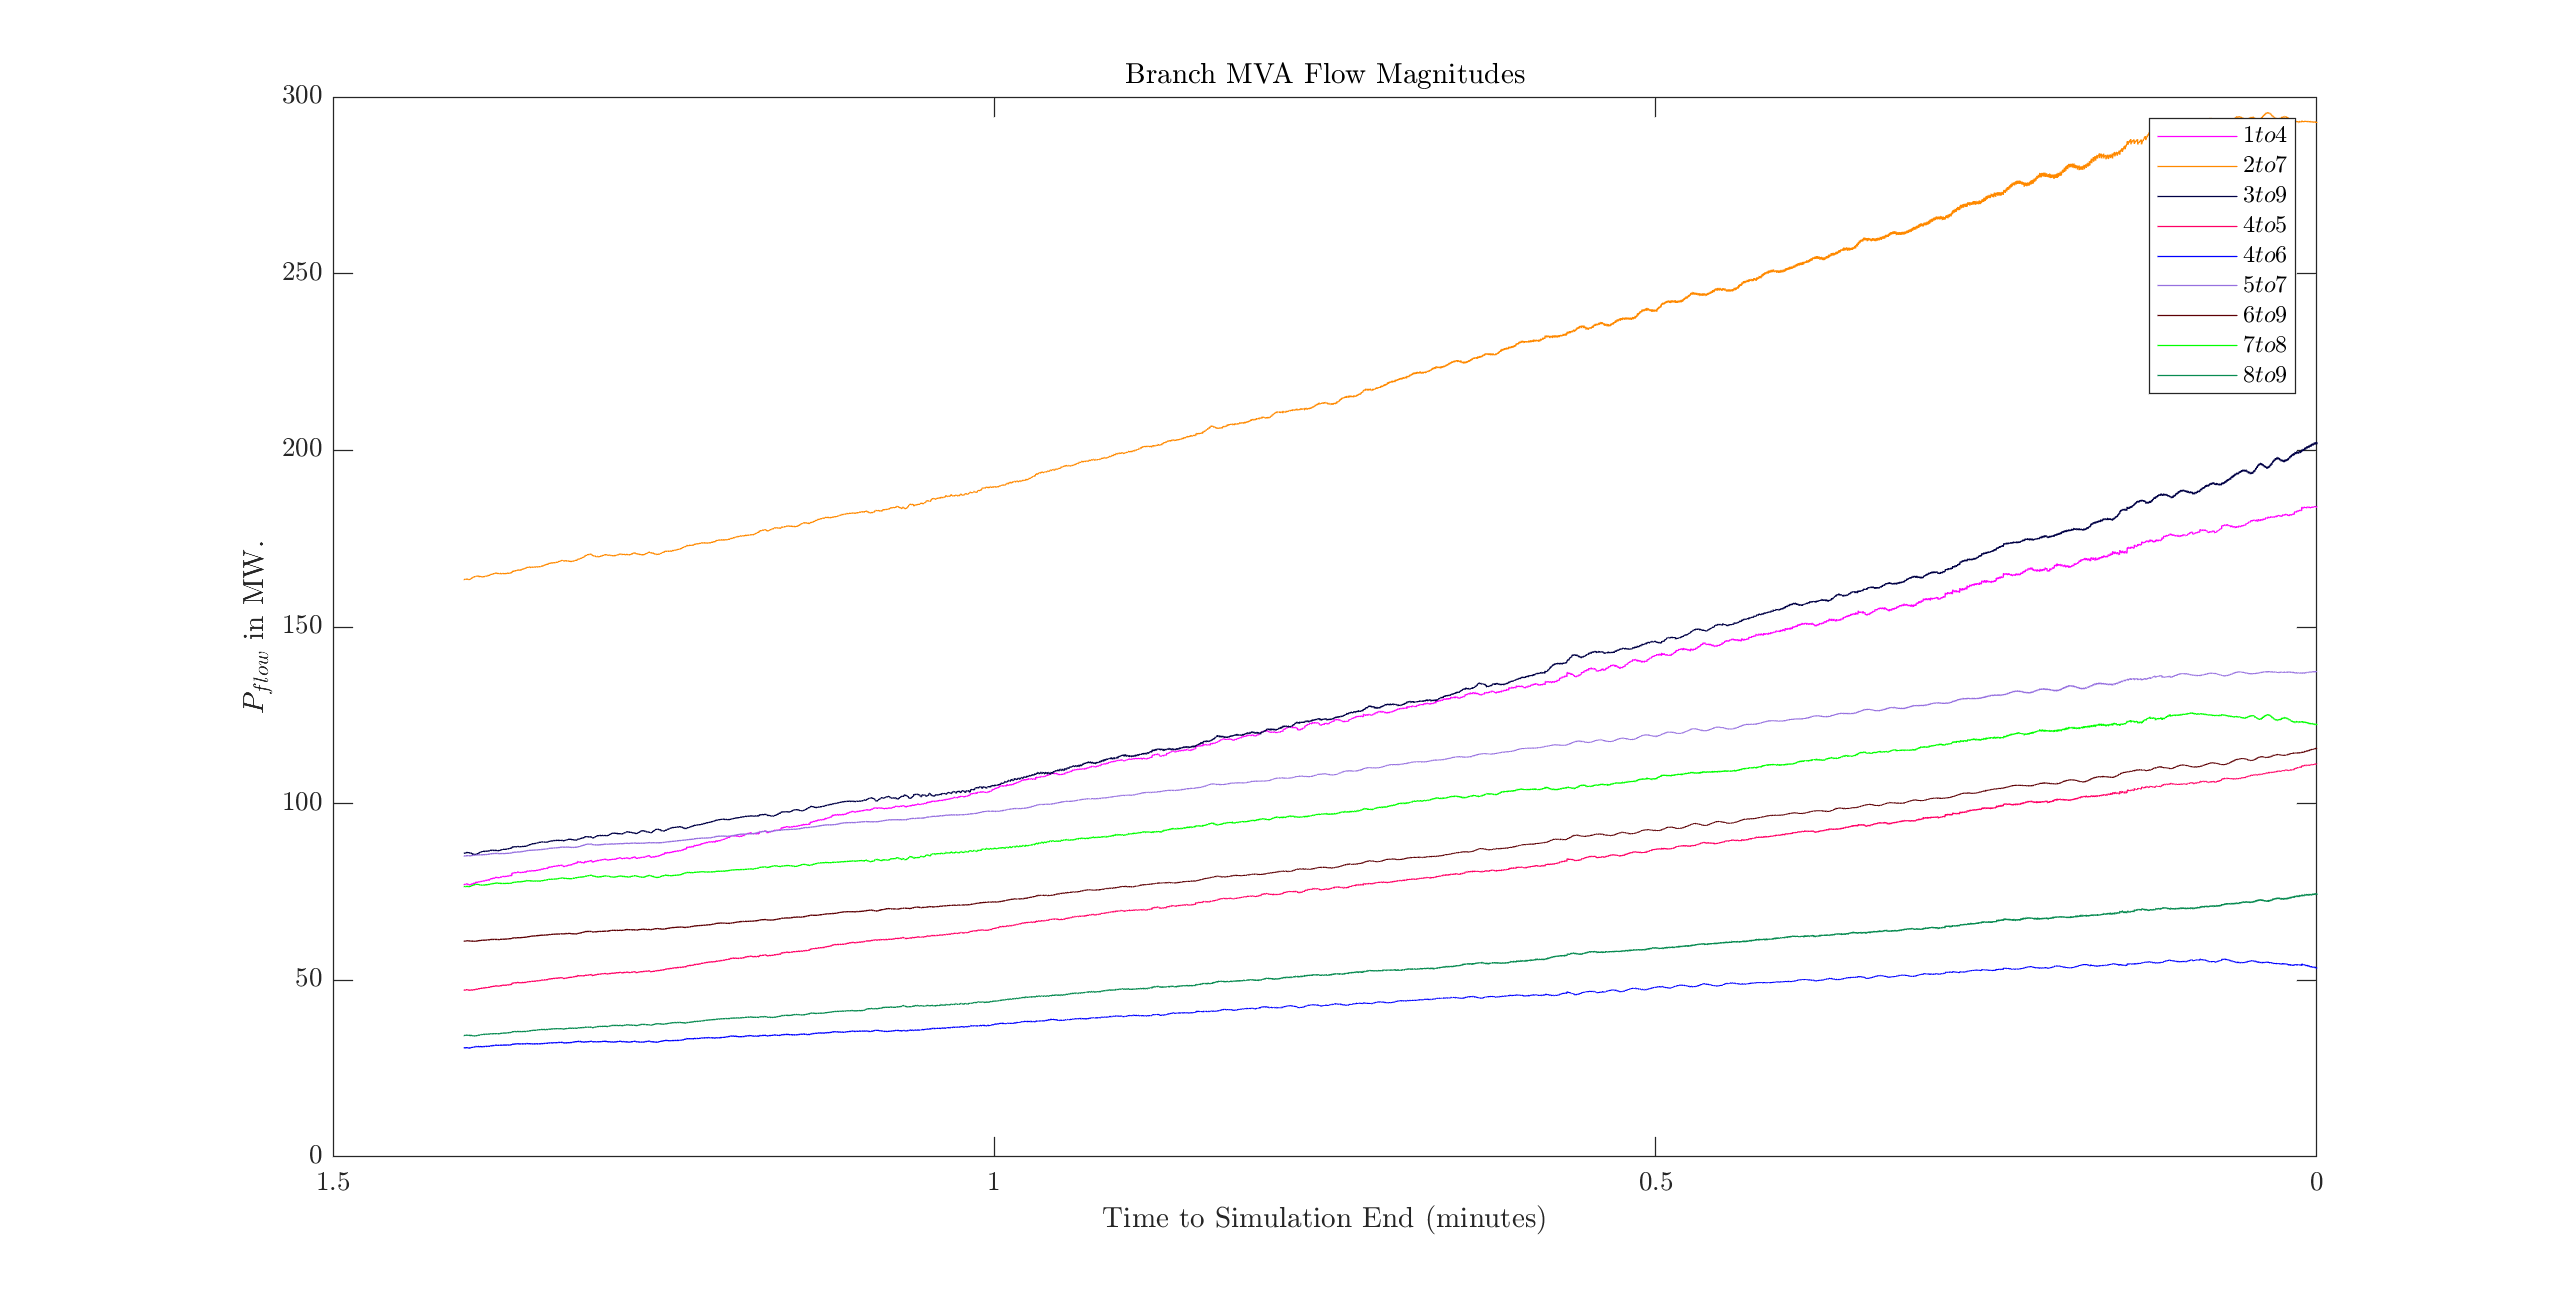
\includegraphics[scale=0.25]{../figures/analysis_matlab/currents_run02}
		\caption{Line Currents for the simulated IEEE 9 Bus System vs simulation time.}
	\end{subfigure}
	
	\begin{subfigure}{\textwidth}
		\centering
		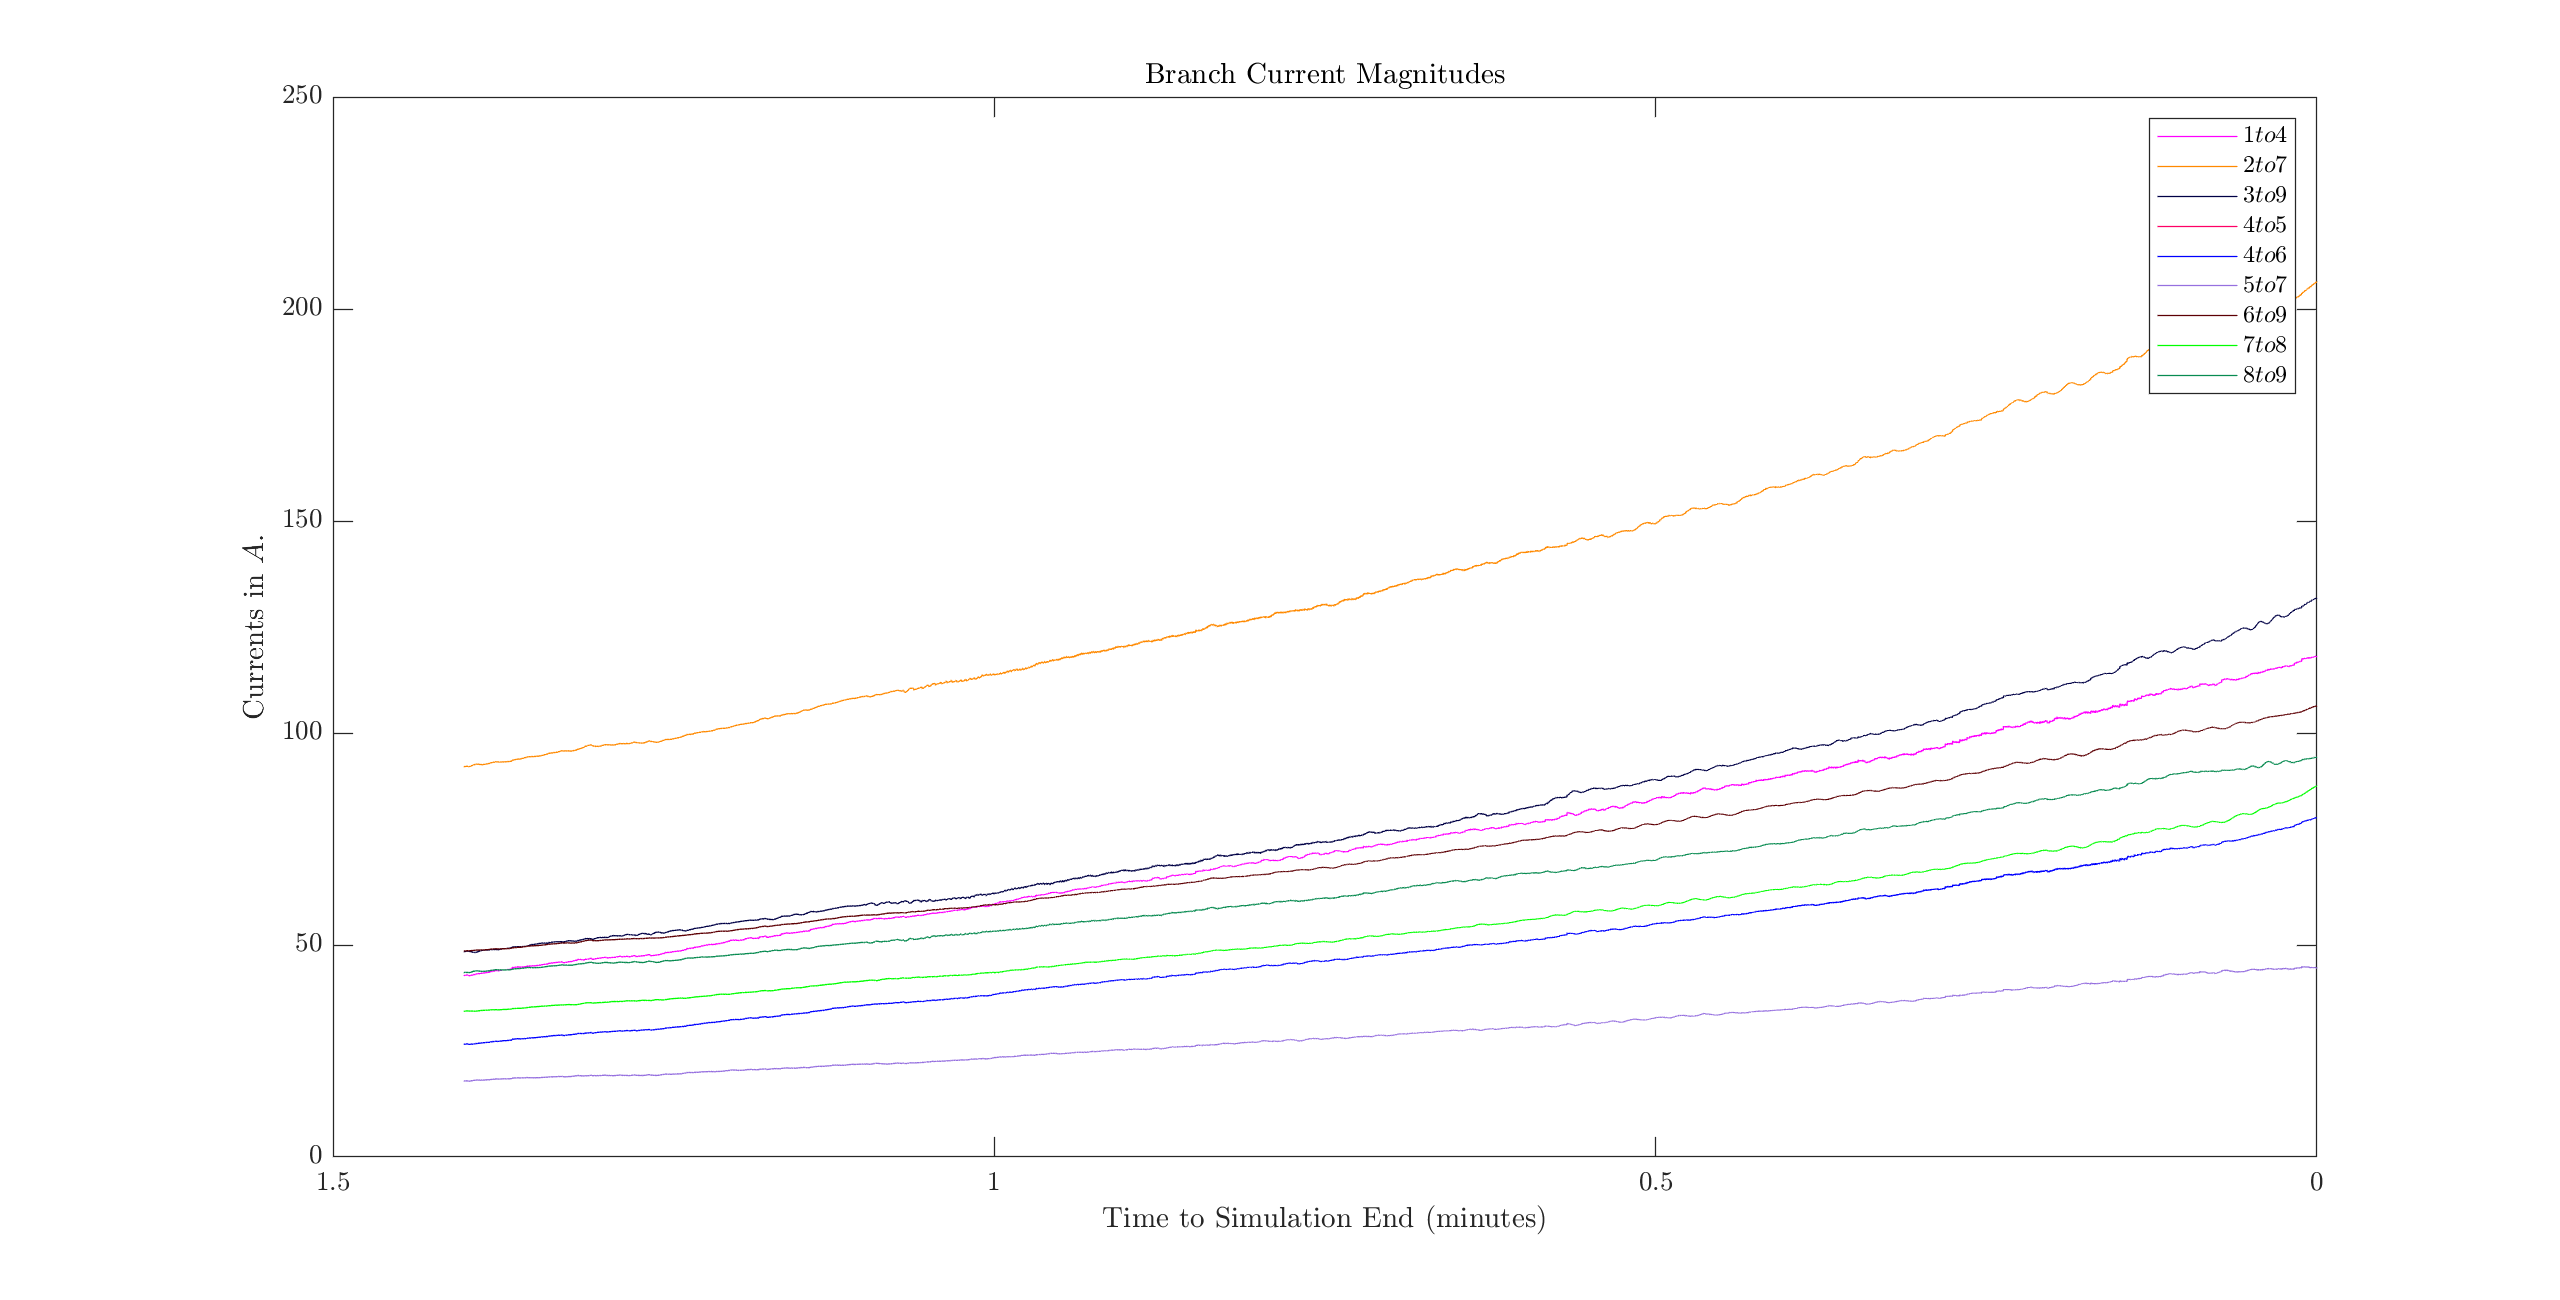
\includegraphics[scale=0.25]{../figures/analysis_matlab/mvas_run02}
		\caption{Line MVAs for the simulated IEEE 9 Bus System vs simulation time.}
	\end{subfigure}

	\caption{Simulation results of the IEEE 9 Bus System as per the prescribed conditions.}
\end{figure}

\begin{figure}[!htpb]
	\centering
	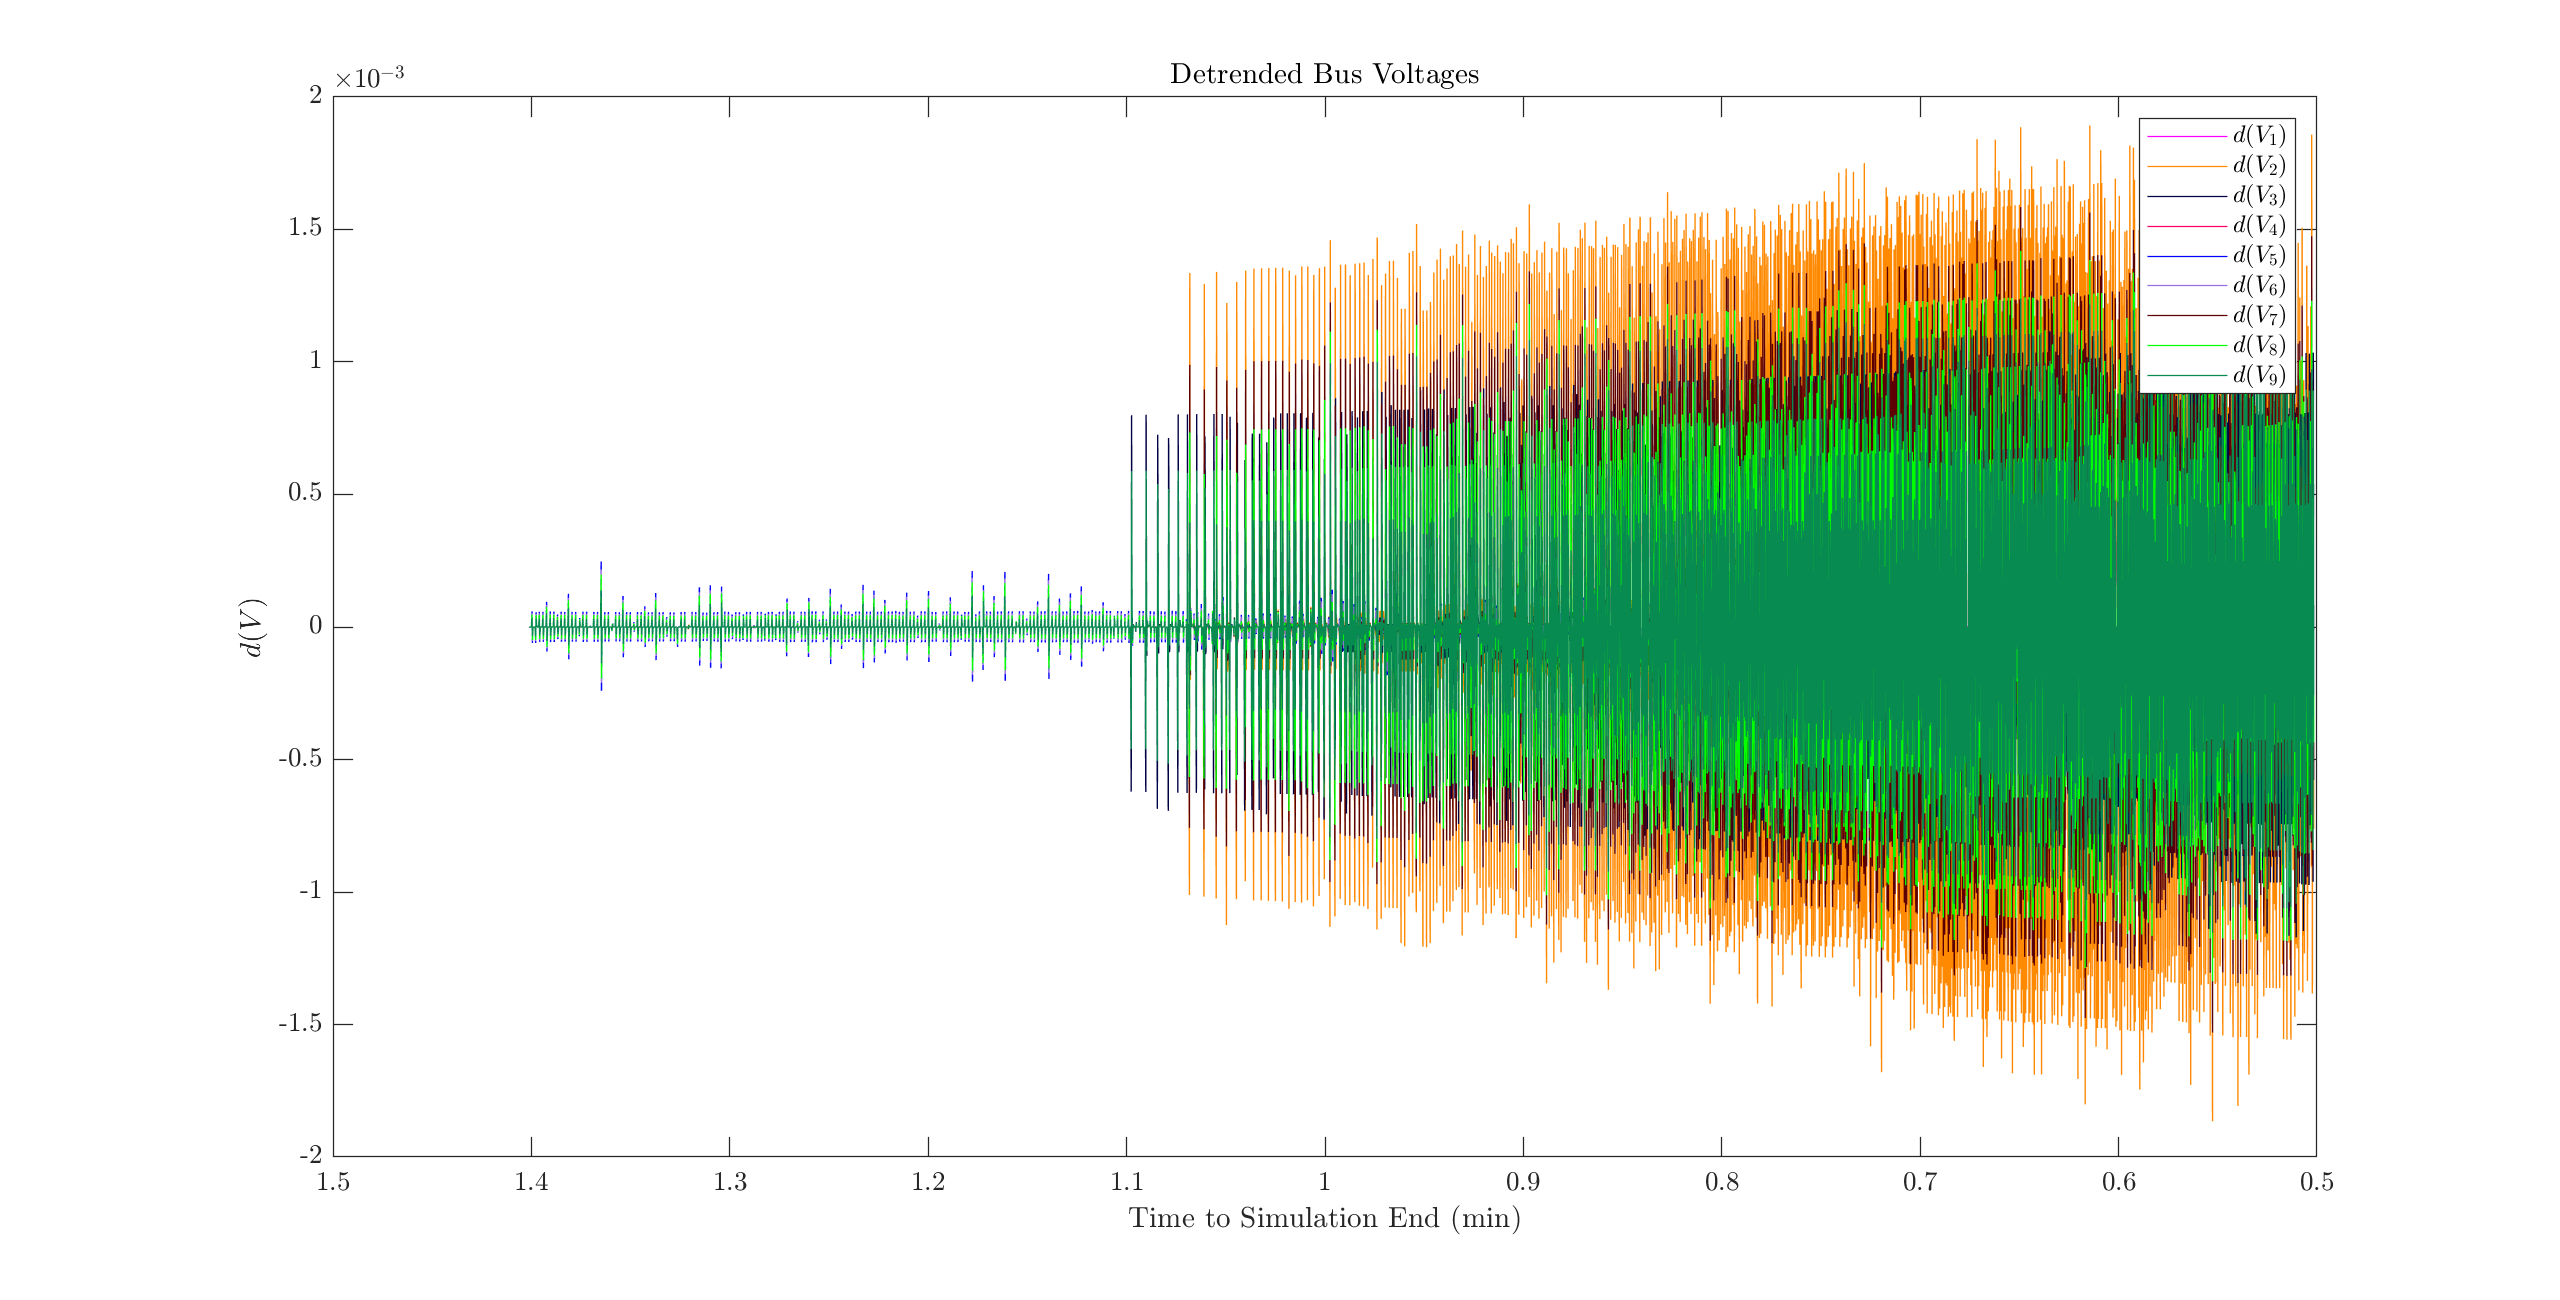
\includegraphics[scale=0.25]{../figures/analysis_matlab/voltsDetrended_run02}
	\caption{Detrended Bus Voltages for the simulated IEEE 9 Bus System vs simulation time.}
\end{figure}

\begin{figure}[!htpb]
	\begin{subfigure}{\textwidth}
		\centering
		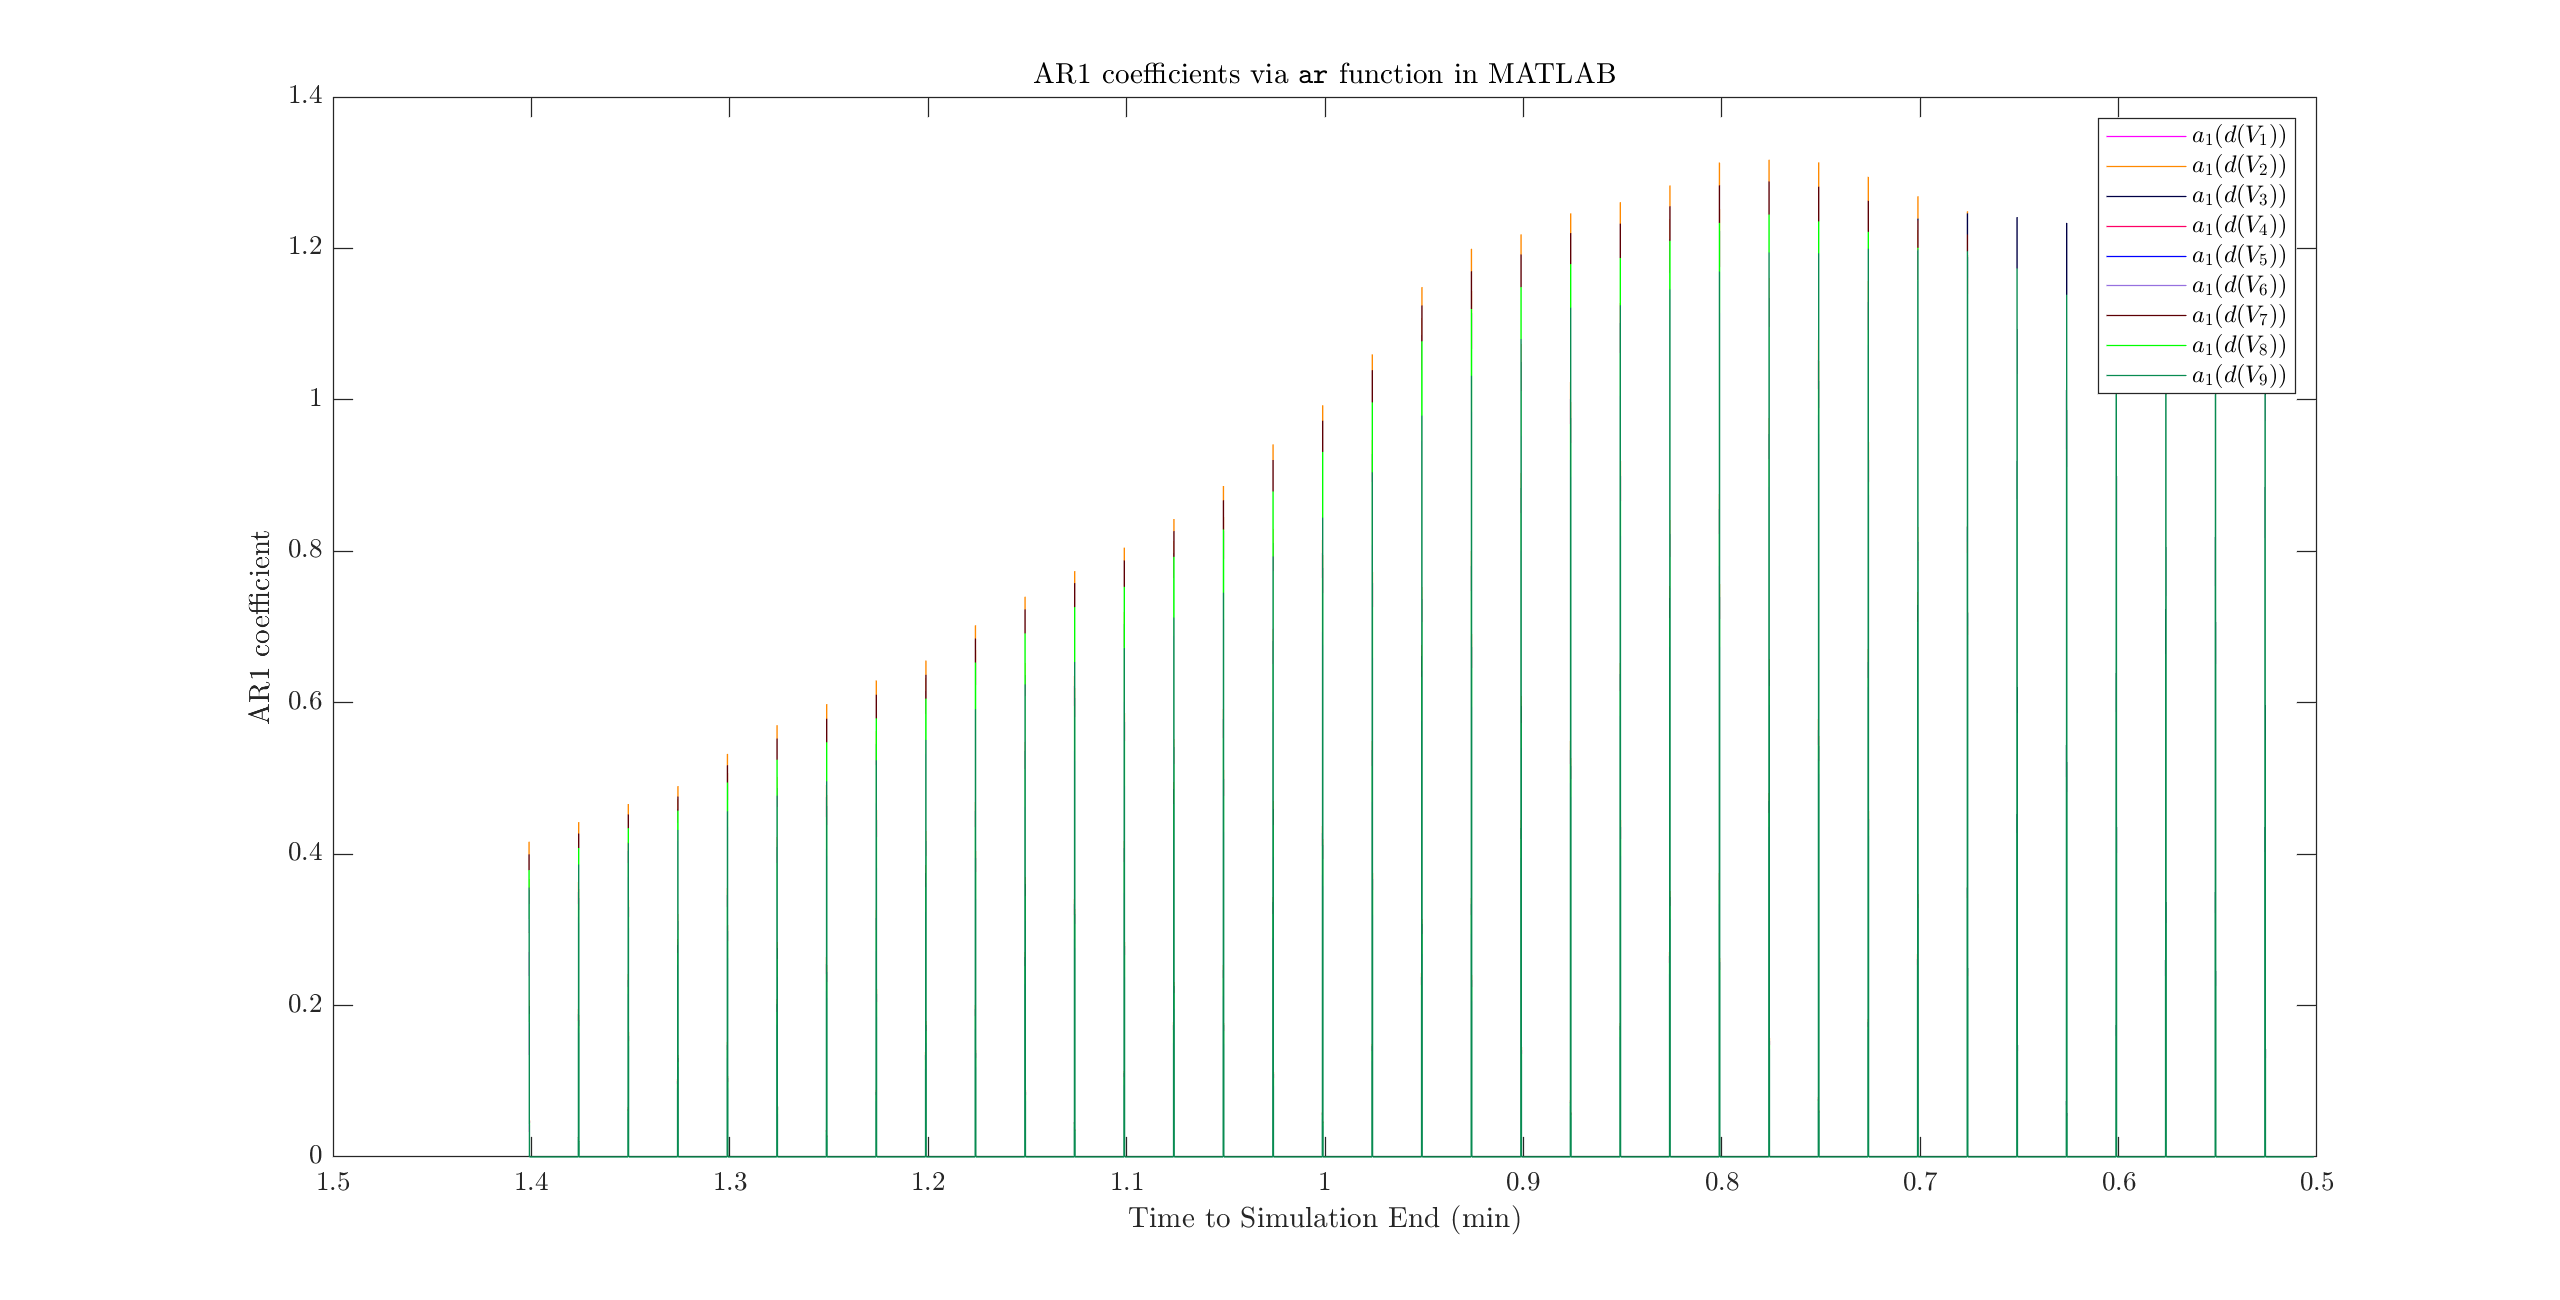
\includegraphics[scale=0.25]{../figures/analysis_matlab/ar1_run02}
		\caption{Fixed Lag Autocorrelations with Lag $\tau = 1s$ computed for the Detrended Bus Voltages for the simulated IEEE 9 Bus System vs simulation time.}
	\end{subfigure}
	
	\begin{subfigure}{\textwidth}
		\centering
		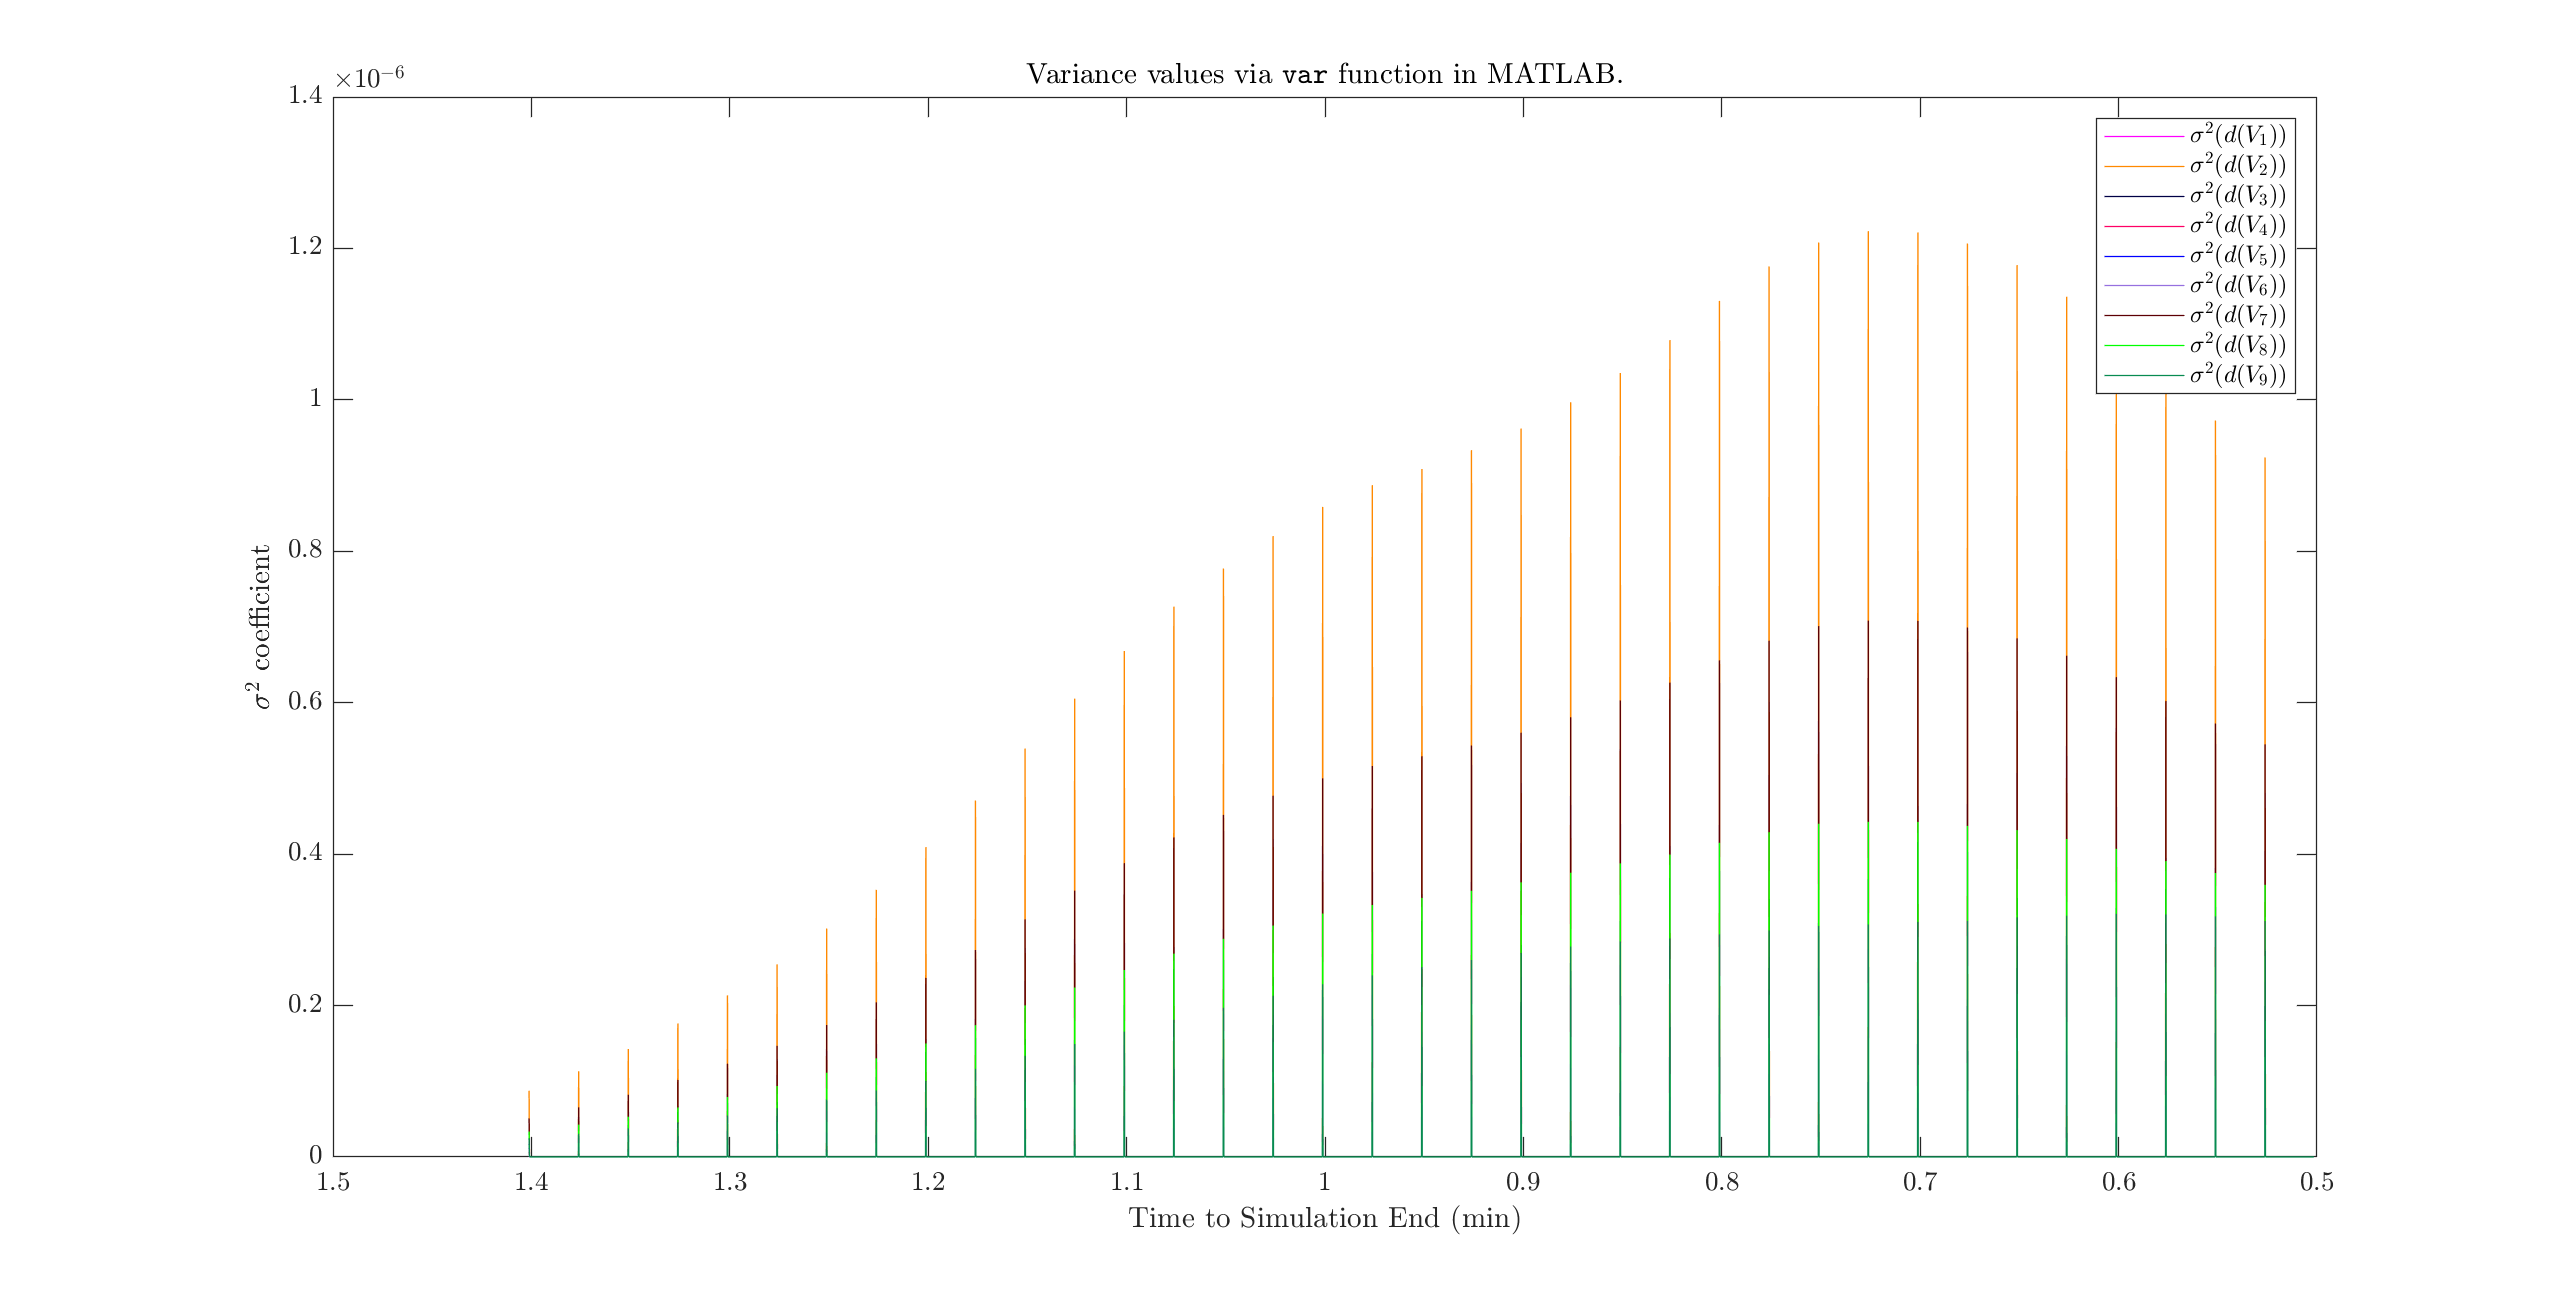
\includegraphics[scale=0.25]{../figures/analysis_matlab/var_run02}
		\caption{Variances computed for the Detrended Bus Voltages for the simulated IEEE 9 Bus System vs simulation time.}
	\end{subfigure}
	
	\caption{Data Analysis done on the Bus Voltages resulting from the IEEE 9 Bus System Simulation for the purpose of testing if the system shows symptoms of Critical Slowing Down.}
\end{figure}

\begin{figure}[!htpb]
	\begin{subfigure}{\textwidth}
		\centering
		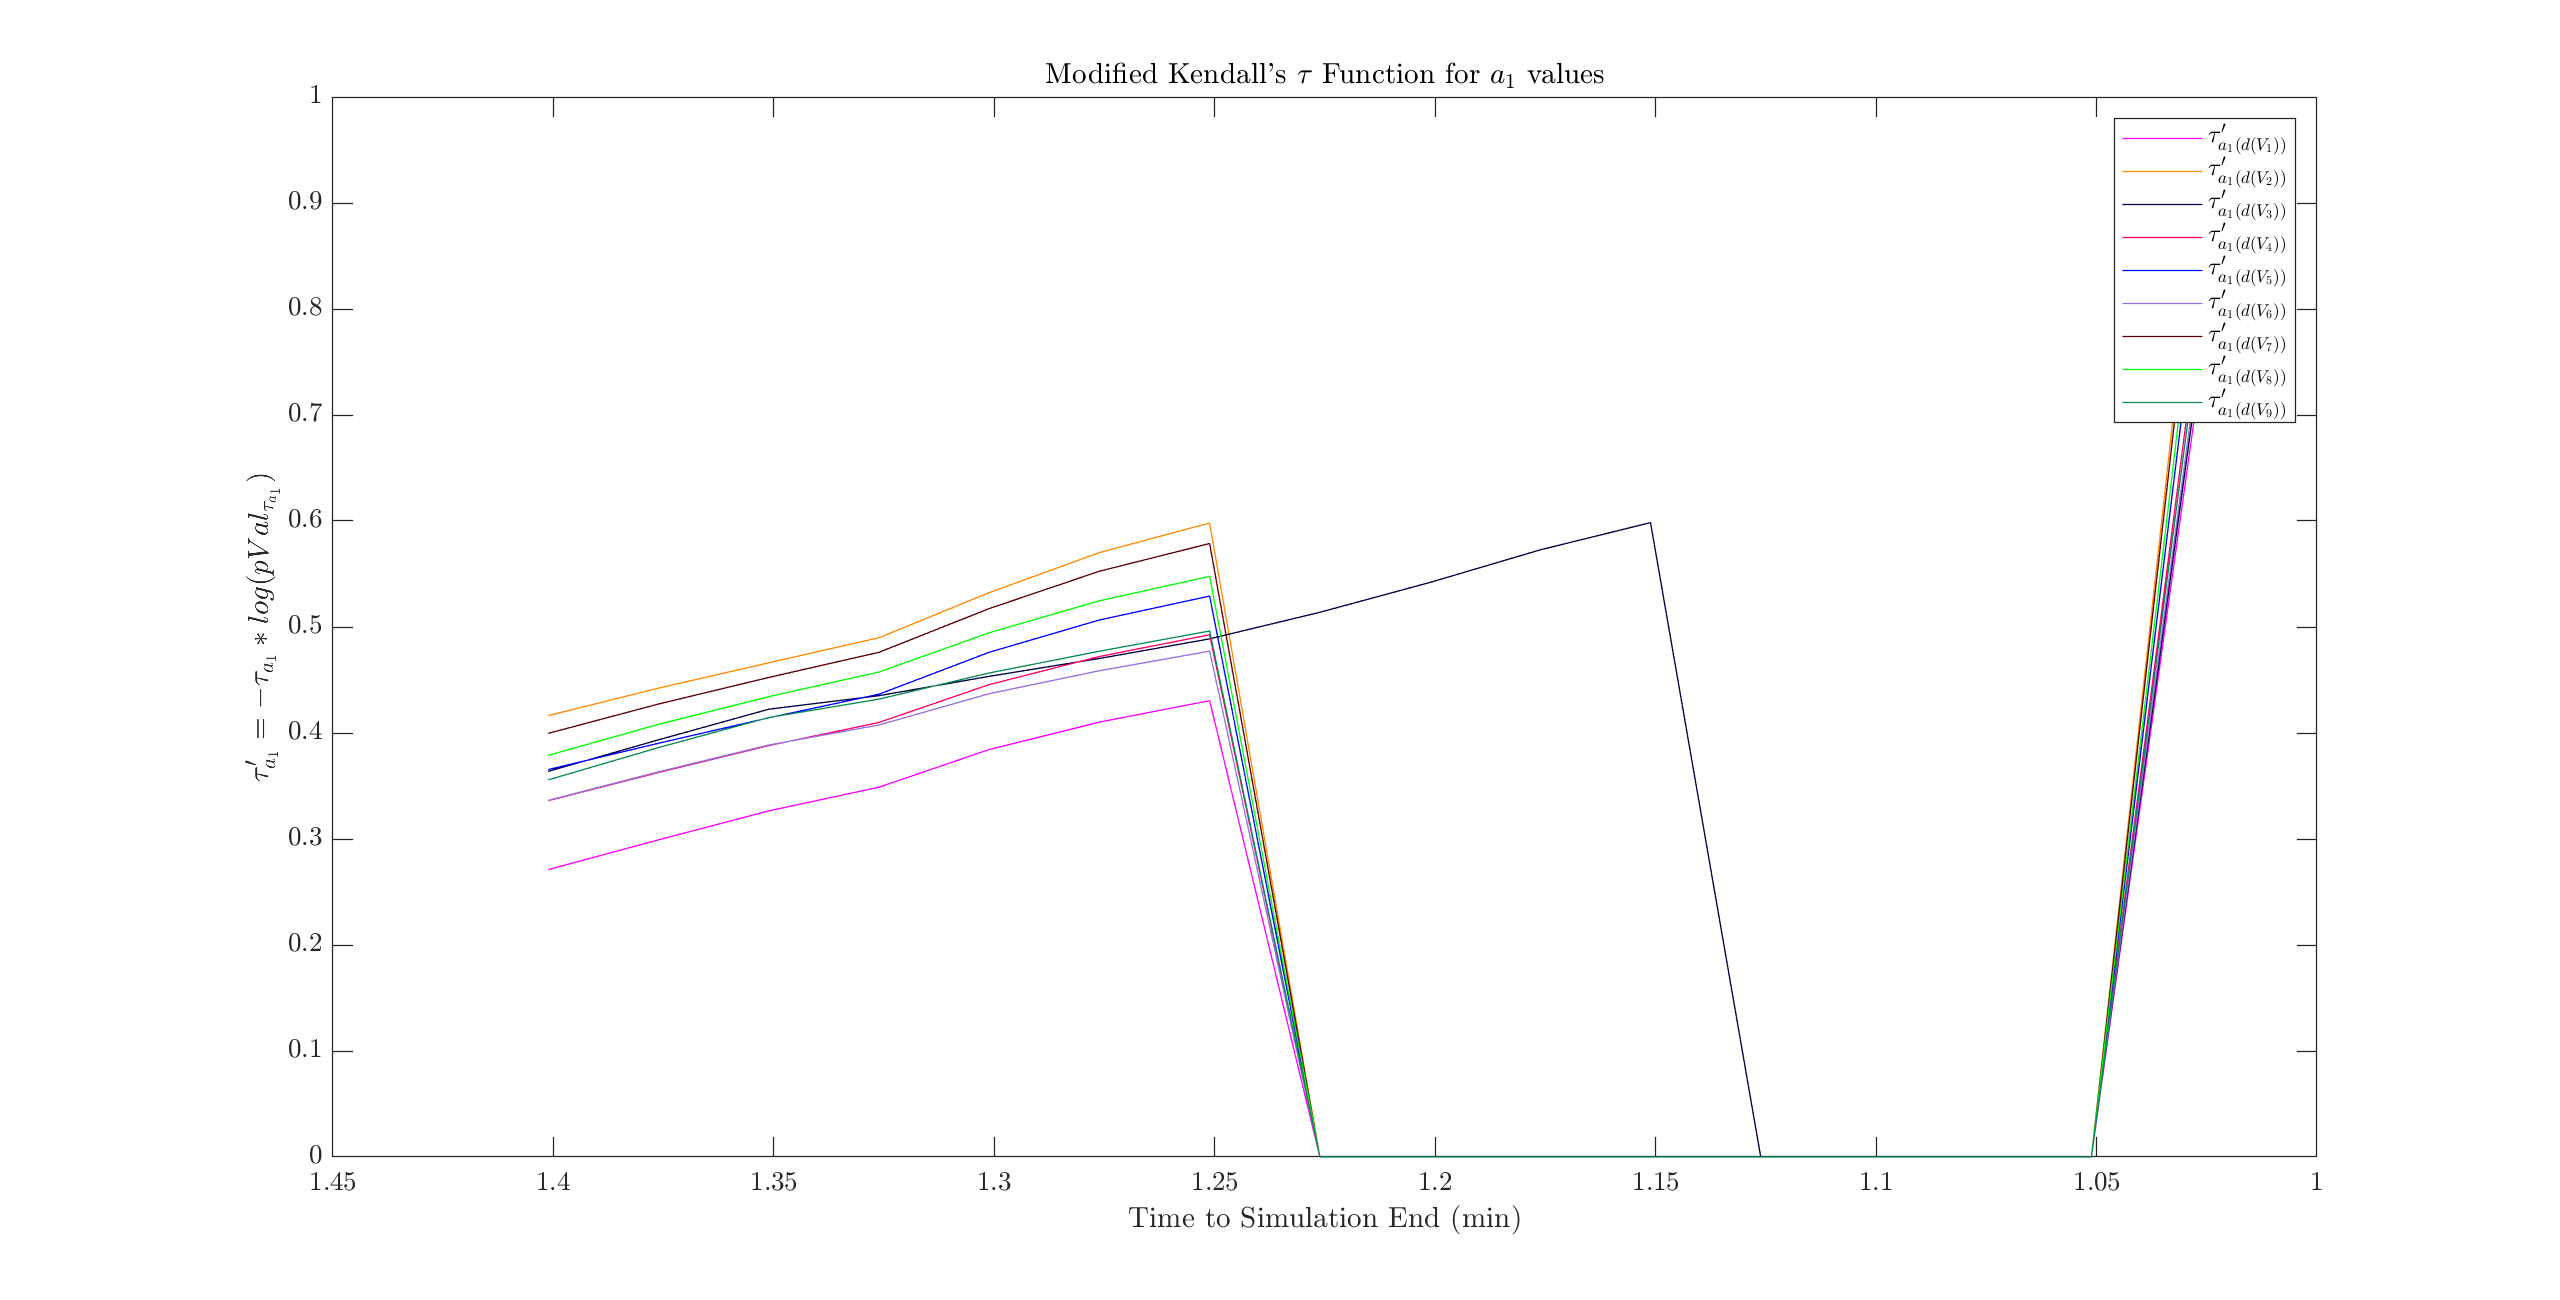
\includegraphics[scale=0.25]{../figures/analysis_matlab/mktcc_ar1_run02}
		\caption{Modified Kendall's Tau Correlation Coefficients (MKTCC) computed for the previously computed Fixed Lag Autocorrelations of the Detrended Bus Voltages.}
	\end{subfigure}
	
	\begin{subfigure}{\textwidth}
		\centering
		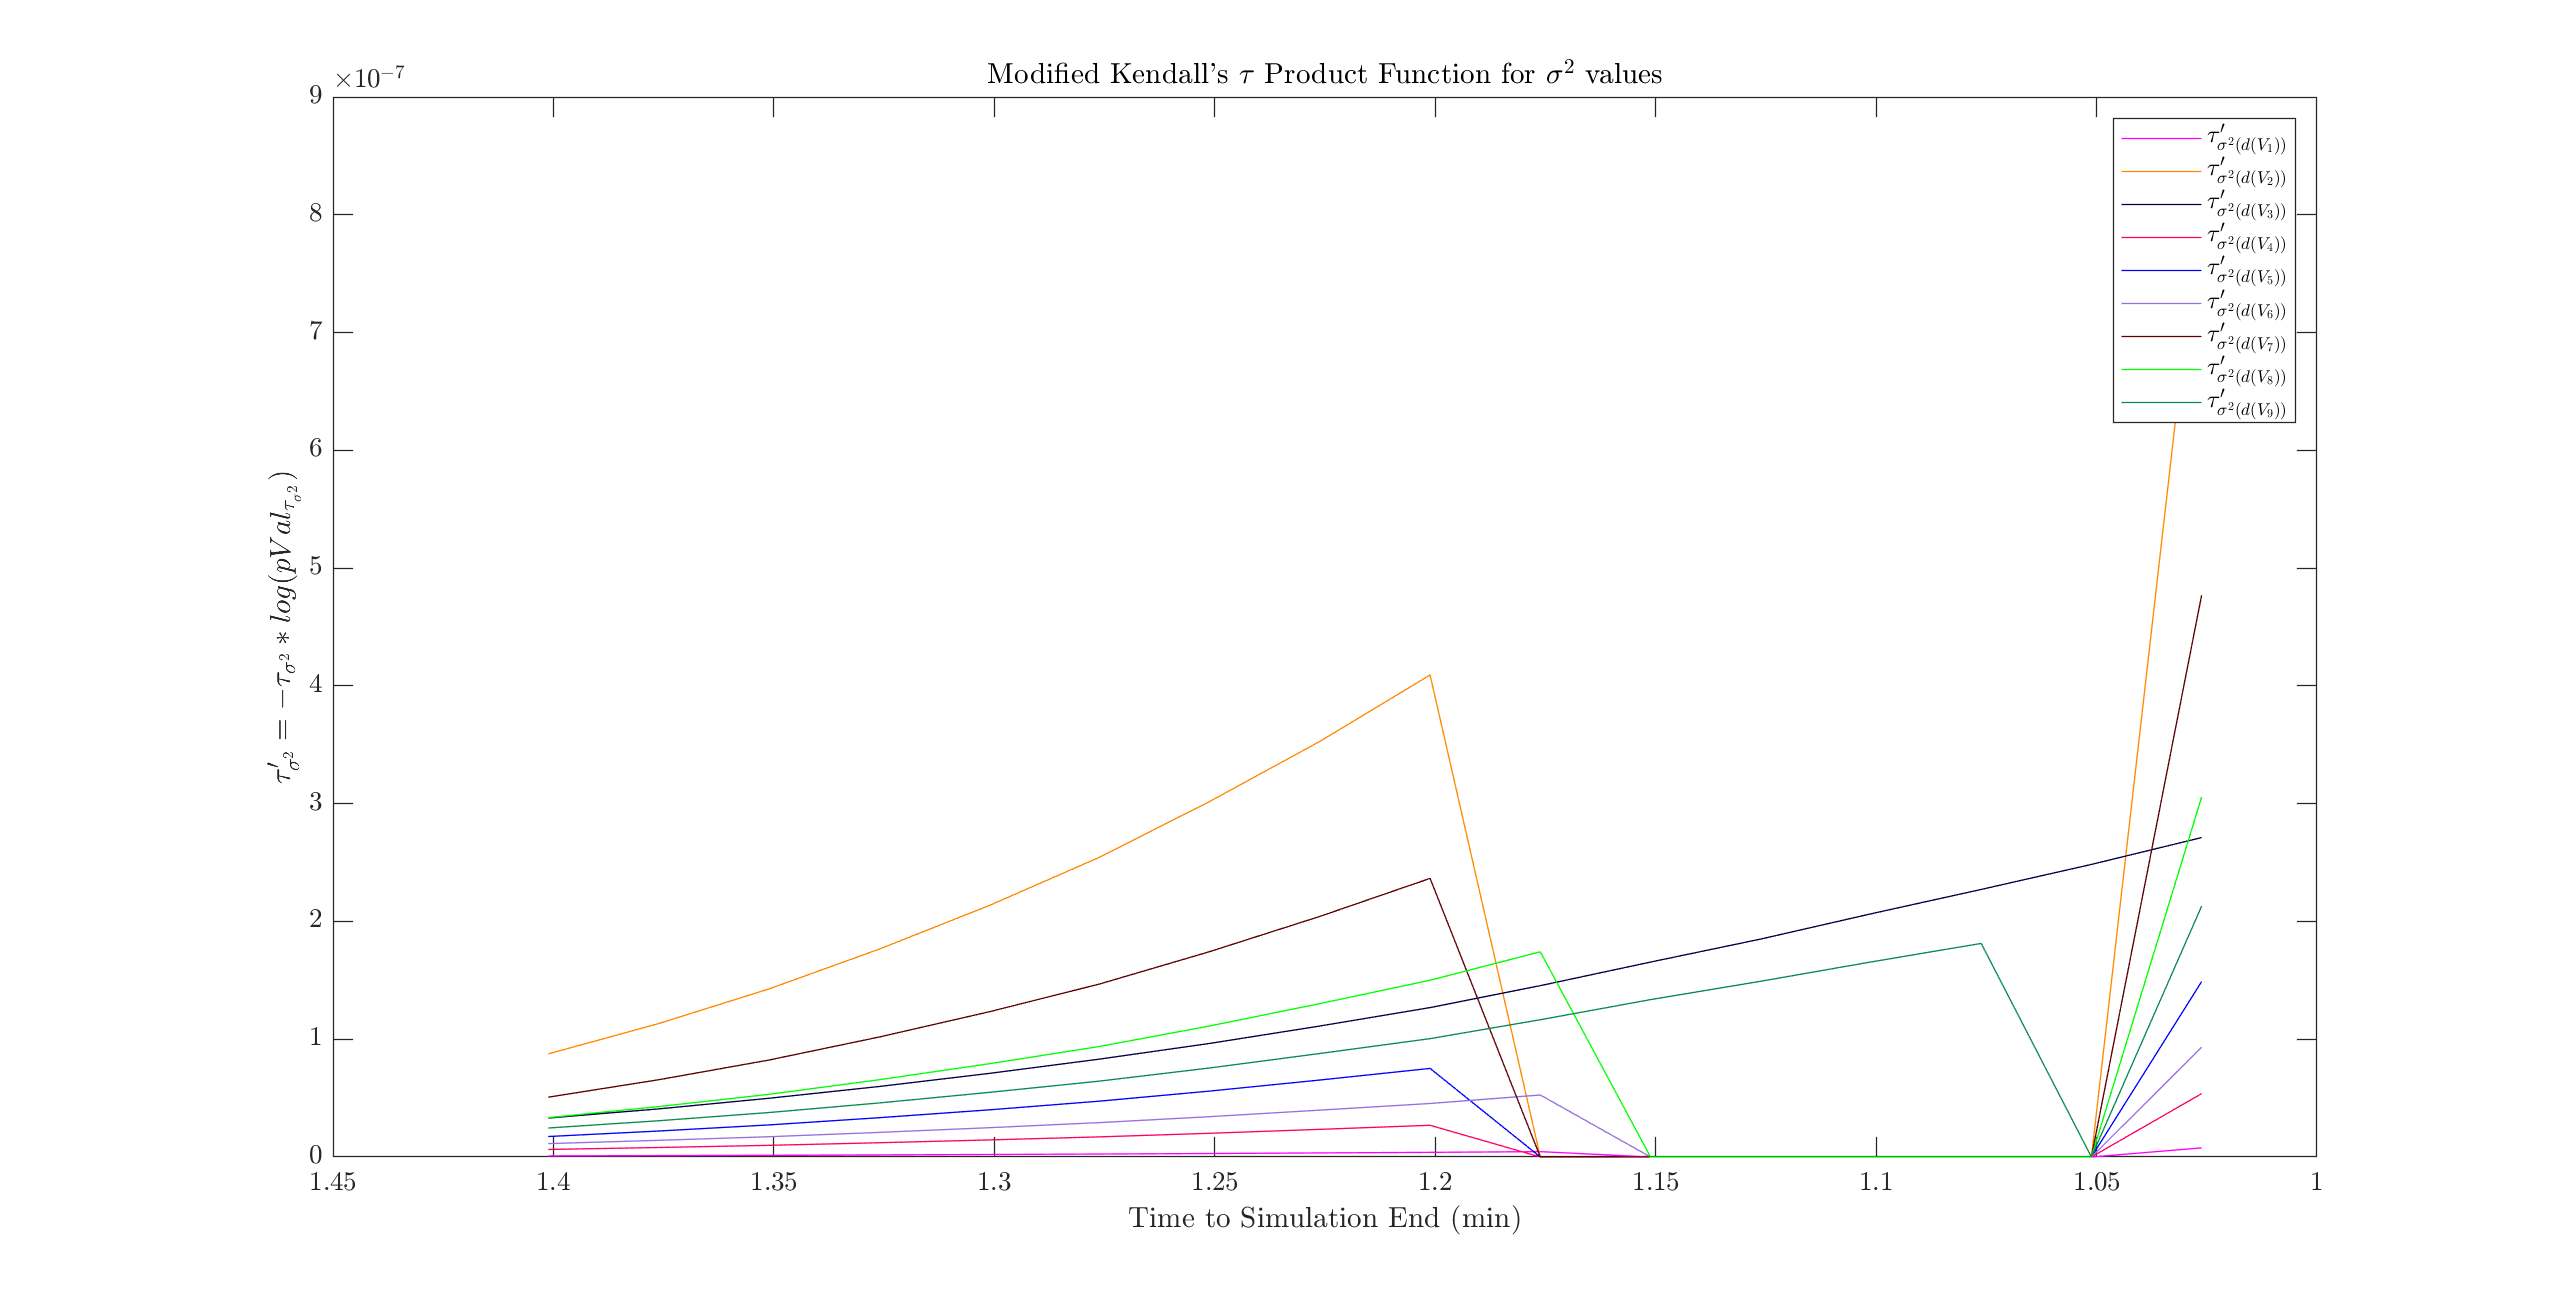
\includegraphics[scale=0.25]{../figures/analysis_matlab/mktcc_var_run02}
		\caption{Modified Kendall's Tau Correlation Coefficient (MKTCC) computed for the previously computed Variances of the Detrended Bus Voltages.}
	\end{subfigure}
	
	\caption{Modified Kendall's Tau Correlation Coefficient was used for checking for any serial dependence of the autocorrelation and variance data, i.e. if the increases in both parameters was statistically significant or not.}
\end{figure}

It should be noted that while autocorrelation was used in both online/real-time (as Fixed Lag Autocorrelation) and offline/postmortem analyses (as Fixed Time Autocorrelation), the two usages were different in:

\begin{itemize}
	\item their mode of procuring and processing input data (a running window of an incoming stream of data vs previously stored months/years worth of time series),
	\item the degrees of freedom allowed for its two parameter variables (which out of $t$ and $\tau$ is allowed to be constant),
	\item their theoretically expected output data (autocorrelation is should decrease exponentially with respect to time lag $\tau$ but increase with time $t$ if that the system is being progressively stressed with time)
\end{itemize} 
 
 